\chapter{NECTA Past Problems}

\section{Form I}
	\subsection{Numbers, Fractions, Decimals, Approximations}
	
\begin{enumerate}


			\subsubsection{Evaluation / BODMAS}
%evaluate (BODMAS)
	\item Evaluate $[9876 - 4321] \div 55 - 7 \times 6 + 3$
	
	\item Evaluate $24 \times (10 + 54) \div 8 - 2$
	
	\item Using mathematical tables, evaluate $\cfrac{(36.12)^3 \times 750.9}{(113.2)^2 \times \sqrt{92.5}}$
	
%fraction form	 	
	 \item Evaluate $\cfrac{ \frac{1}{25} + 0.28 + 1\frac{17}{25} }{ 3\frac{1}{5} \div \frac{0.32}{0.15} }$ Give your answer in fraction form.
	 
	 \item Evaluate $\cfrac{0.0084 \times 1.23 \times 3.5}{2.87 \times 0.056}$ with using mathematical tables and express the answer as a fraction in its simplest form.

%numbers - standard form
	\item Given $x = 4.5 \times 10^{-7}$ and $z = 7.2 \times 10^5$, find $y$ in standard form if $z = xy$.
	
	\item Given $x = 1.6 \times 10^8$ and $y = 5.6 \times 10^4$, find $z$ in standard form if $ xz = y$.
	
	\item Compute $0.678 \times 145$ and express the answer in standard form.
	
	\item Given that $M = 4 \times 10^3$, express $\frac{1}{M}$ in standard form.


			\subsubsection{GCF, LCM}
%GCF, LCM	
	\item Find the product of the LCM and GCF of 40, 120 and 240.
	
	\item Find (a) GCF and (b) LCM of 15, 35 and 56.
	
	\item Two numbers, 60 and $n$, have the lowest common multiple (LCM) of 420. If $n$ is a multiple of 6 less than 90, find:
		\begin{itemize}
		\item[(i)] the possible values of $n$.
		\item[(ii)] the greatest common factor (GCF) of the two numbers.
		\end{itemize}	
		
	\item The GCF and LCM of $y$, 18 and 60 are 6 and 360 respectively. Find the value of $y$.
		
	\item The numbers 28, 41, 42, 59, 70 belong to the set of natural numbers. By using these numbers:
		\begin{itemize}
		\item[(i)] calculate the difference between the least common multiple (LCM) of the prime numbers and the greatest common factor (GCF) of the remaining numbers.
		\item[(ii)] express the answer obtained in (i) above in the standard form $A \times 10^n$ correct to two significant figures where $1 \leq A < 10$ and $n$ is an integer.
		\end{itemize}			 
	
	
			\subsubsection{Integers}
%integers
	\item By using properties of integers, give reasons why each of the following expressions are equal:
		\begin{itemize}
		\item[(i)] $(15 \times 17) \times 12 = 17 \times (15 \times 12)$
		\item[(ii)] $15 \times (17 + 12) = (15 \times 17) + (15 \times 12)$
		\end{itemize}
		
	\item An aeroplane traveling at an altitude of 3200 metres makes a climb of 1500 metres, followed by a drop of 100 metres.
		\begin{itemize}
		\item[(a)] Represent the plane's altitude as a sum of positive and negative integers.
		\item[(b)] What is the planes altitude after the drop?
		\end{itemize}
	

		\subsubsection{Recurring Decimals}	 
%recurring decimals
	 
	 \item Express $1.8\dot{6}$ as an improper fraction in its simplest form.
	 
	 \item Change $0.\dot{1}2\dot{3}$ into a fraction.
	 
	 \item Express $23.\dot{1}2\dot{3}$ as a fraction.
	 
	 \item Express $2.\dot{1}35\dot{3}$ as a fraction.
	 
	 \item Express $2.\dot{1}4\dot{6}$ as a fraction.
	 
	 \item Change $0.0\dot{1}$ into a fraction.
	 
	 \item Determine the fractional notation for $0.6\dot{3}$.
	 
	 \item Express $1.\dot{2}1\dot{3}$ as a rational number.
	
	\item Express the following recurring decimal number as a rational number: $0.\dot{6}5\dot{7}$.
	 
	 \item Express $0.8\dot{3}$ in the form $\frac{a}{b}$ where $a$ and $b$ are integers such that $b \neq 0$.
	 
	 \item Express $0.\dot{3}0\dot{3}$ as a fraction, i.e. $\frac{a}{b}$ where $a$ and $b$ are integers and $b \neq 0$.

			\subsubsection{Word Problems}
	\item Mr. Bean lived a quarter of his life as a child, a fifth as a teenager and a third as an adult. He then spent 13 years in his old age. How old was he when he died?	
			
	\item Mary received a certain amount of money from her father to go to school. She spent one third in her journey to school. At school she paid two thirds of the remaining amount as school fees and remained with 24,000 /= as her pocket money. Showing the procedure, calculate the total amount of money she received from her father. 
			
	\item A certain worker used his salary as follows: 20\% on house rent, 45\% on food, 10\% on refreshment and 15\% on school fees. If he\slash she was left with Tsh. 22,000, determine:
		\begin{itemize}
		\item[(i)] the salary of the worker.
		\item[(ii)] the amount of money which he\slash she spent on food.
		\end{itemize}

		\subsubsection{Approximations}	
%approximations - give to _ decimal places
	\item By using mathematical tables, evaluate $\cfrac{\sqrt[3]{0.0072} \times (81.3)^2}{\sqrt{23140}}$ to three significant figures.
	
	\item By using mathematical tables, evaluate $\cfrac{(28.32)^4 \times 0.03574}{87.57}$. Give your final answer in standard form, to three significant figures.
	
	\item If $a = 2.432 \times 10^4$, $b = 7.42 \times 10^{-2}$ and $c = 0.0324 \times 10^{-2}$, find the value of $R$ in standard form correct to two decimal places given that $R = \cfrac{ab}{c}$.
	
	\item Using mathematical tables, evaluate the expression: $\cfrac{(28.32)^2 \times 0.3574}{\sqrt{8.732}}$. Give the answer correct to four decimal places.
	 
	 \item By using mathematical tables evaluate the expression $\cfrac{237.8 \times 0.0873}{67890}$. Give the answer to four figures.
	 
	 \item Given that $\sqrt{3} = 1.7321$, calculate the value of $\cfrac{2}{\sqrt{3} - 1}$ correct to 4 decimal places.

%round off, estimate
	\item Estimate he value of $\cfrac{57.2 \times 110}{2.146 \times 46.9}$ correct to one (1) significant figure.
	 
	 \item 
	 	\begin{itemize}
	 	\item[(a)] Find the value of the expression $\left(\cfrac{4.75 + 1.31}{3.13}\right)^2$ giving your answer in three decimal places.
	 	\item[(b)] By rounding each term of the expression in (a) above to one significant figure, obtain a rough estimate of the expression.
	 	\end{itemize}
	 
	 \item 
	 	\begin{itemize}
	 	\item[(a)] Round off each of the following numbers to one decimal place. $L = 20.354$, $M = 40.842$, $N = 10.789$
	 	\item[(b)] Use the result obtained in (a) above to find the value of $x$ given that $x = \cfrac{LM}{N}$.
	 	\end{itemize}
	 	
	\item Round each of the numbers $x = 2.354$, $y = 4.843$ and $z = 1.789$ to one decimal place and then use the results obtained to find the value of $A$ to two significant figures given that $A = \cfrac{xy}{z}$.
	 
	\item Express 0.05473
		\begin{itemize}
		\item[(i)] correct to three (3) significant figures
		\item[(ii)] correct to three (3) decimal places
		\item[(iii)] in standard form
		\end{itemize}
	
	\item Write 624.3278 correct to
		\begin{itemize}
		\item[(i)] five significant figures
		\item[(ii)] three decimal places
		\end{itemize}



\end{enumerate}	

	\subsection{Geometry}
	
\begin{enumerate}
		\item 
		\begin{itemize}
		\item[(i)] What is the sum of the interior angles of an octagon?
		\item[(ii)] Find the size of the exterior angle of a regular octagon.
		\end{itemize}
		
	\item Calculate the size of an interior angle of a regular nonagon.
	
	\item A regular polygon has an exterior angle of $36^\circ$. Calculate:
		\begin{itemize}
		\item[(a)] the size of an interior angle
		\item[(b)] the number of sides of the polygon
		\end{itemize}
	
	\item An exterior angle of a regular polygon has degree measure of 22$^1/_2$. Find the sum of degree measure of all the interior angles.
	
	\item The interior angle of a regular polygon is $120^\circ$ greater than the exterior angle. Find the number of sides of the polygon.
	
	\item If the interior angle of a regular polygon is $6^1/_2$ times the exterior angle, how many sides does the polygon have?


\end{enumerate}

	\subsection{Algebra}
	
	See Form II \nameref{f2algebra}.

	\subsection{Ratio, Profit and Loss}
\begin{enumerate}

		\subsubsection{Ratio}
	\item An alloy consists of three metals A, B and C in the proportions $A:B = 3:5$ and $B:C = 7:6$. Calculate the proportion $A:C$.		
		
	\item Given the ratios:\\
	$A : B = 2 : 3$\\
	$B : C = 6 : 7$\\
	Calculate the ratio of $A : C$.
	
	\item Express $2\frac{1}{2} : 3$ as integers in a simplified form.
	
	\item If it is known that $x:y = 5:1$ find the value of $\cfrac{x + y}{3x - 4y}$.
	
	\item Three numbers $d$, $m$ and $n$ are in the ratio of $3:6:4$ respectively. Find the value of $\cfrac{4d - m}{m + 2n}$.
	
	\item A, B and C are to share Tshs. 120,000/= in the ratio $2:3:5$ respectively. How much will each get?
	
	\item Three people share a property in the ratio $2:x:y$. It is known that $y = x + 2$. If the largest shareholder had Tsh. 39,100/= in monetary terms, find the value of this property.
	
	\item The ratio of men : women : children living in Mkuza village is 6 : 7 : 3. If there are 42,000 women, find how many:
		\begin{itemize}
		\item[(a)]
			\begin{itemize}
			\item[(i)] children live in Mkuza village.
			\item[(ii)] people altogether live in Mkuza village.
			\end{itemize}
		\item[(b)] The 42,000 women is an increase of 20\% on the number of women ten years ago. How many women lived in the village?
		\end{itemize}
		
	\item An amount of Tshs. 12,000 is to be shared among Ali, Anna and Juma in the ratio 2 : 3 : 5 respectively. How much will each get?

	\item The are of two circles are in the ratio of 16 : 9. Calculate the radius of the smaller circle when the radius of the larger one is 24 cm.
	
	\item The ratio of the areas of two circles is 50 : 72. If the radius of the smaller circle is 15 cm, find the radius of the larger circle.
	
	\item The sides of a rectangle are in the ratio 3 : 5. If the perimeter of this rectangle is 800 cm, find the dimensions of the rectangle.
	
	\item The distance between two towns on a map of scale 1 : 5,000,000 is 9 cm. Find the actual distance between the towns in kilometres.
	
	\item A building 250 metres high is represented by a line segment of length 5 cm. Find the scale of drawing.
	
	\item An area of 24.7 cm$^2$ was plotted on a map of a scale 1 : 50,000. What was this area, in square kilometres, on the Earth's surface?
	
	
		\subsubsection{Profit and Loss}
%profit and loss
	\item 
		\begin{itemize}
		\item[(a)] John and Paul started a tailoring business and invested shs 110,250/= and 220,500/= respectively. If the profit after the first six months was shs 50,970/=, how much did Paul get if they agreed to share it according to the amount they invested.
		\item[(b)] Mary paid shs 800,000/= for a computer and sold it the following year for shs 600,000/=. Find the percentage loss she got.
		\end{itemize}
		
	\item By selling an article at shs. 22,500/= a shopkeeper makes a loss of 10\%. At what price must the shopkeeper sell the article in order to get a profit of 10\%?
	
	\item Neema bought a tray of eggs (containing 30 eggs) for shs. 2,000/=. She boiled the eggs using a litre of kerosene costing shs. 400/= and sold each egg at a price of 100/= each. Find her percentage profit.
	
	\item A shopkeeper sells sugar at sh. 105.00 per kilogram. If he realizes a profit of 5\% over the buying price, find the buying price per kilogram.
	
	
		\subsubsection{Simple Interest}
%simple interest	
	\item Find the amount of money obtained after depositing 900/= for 2 years and 9 months at an annual rate of 6\% simple interest.
	
	\item How long will it take a sum of money to double itself at 5\% per months, simple interest?
	
	\item A certain amount of money was deposited for three years at the annual rate of 5\% simple interest. The interest at the end of the three years was shs. 112.50. Find the principal.
	
	\item For how long should Tshs. 1,200,000/= be invested at simple interest rate of 5\% to get an interest of Tshs. 180,000/=?
	
	\item Mavuno wants to invest lump sum money so that its value after 4 years will be 812,000/=. How much should the investor invest at 4\% per annum single interest?

\end{enumerate}

	\subsection{Coordinate Geometry}

	See Form IV \nameref{f4coordgeo}.
	
	\subsection{Perimeter and Area}

	See Form IV \nameref{f4ap}.

\section{Form II}

	\subsection{Exponents}
\begin{enumerate}
	
	\item Find the value of $x$ for which $2^x \cdot 16 = \cfrac{1}{8^x}$.
	
	\item Solve for $x$ if $2^{x + 1} = 32,768$.
	
	\item Simplify $\cfrac{27^{n + 2} - 6 \times 3^{3n + 3}}{3^n \times 9^{n + 2}}$
	
	\item Solve for $y$ if $\left(\cfrac{1}{9}\right)^{2y} \left(\cfrac{1}{3}\right)^{-y}\div \cfrac{1}{27} = 3^{(-5y)}$
	
	\item If $\left[3^{(x-2)}\right] \left[2^{(3y - 3)}\right] = 72$, find the values of $x$ and $y$.
	
	\item Solve for $x$ if $\left(4^{(x + 3)}\right)\left(16^x\right) = 8^{3x}$

	\item Solve for $x$ if $2^x = 0.25$.
	
	\item Solve the following equations:
		\begin{itemize}
		\item[(a)] $\left(1/3\right)^x = 81^{-1}$
		\item[(b)] $2^{x + 1} = 2^5$
		\end{itemize}
		
	\item Find the value of $t$ in the equation $3^{2t}\left(4^t\right) = 6$.
	
	\item Use the substitution $y = 2^x$ to solve the equation $2^{2x + 1} - 2^{x + 1} + 1 = 2^x$.
	
	\item If $(576)^{m - 4} = 8^m \times 3^m$, find the value of $m$.
	
	\item Solve for $x$ given that $3^{x + 2} - 5 = 76$.
	
	\item If $2^x \times 3^y = 5184$, find $x$ and $y$.
	
	\item Determine the values of $x$ and $y$ from the following expression: $\left(1/2\right)^x(3)^{y - 2} = 432$.
	
	\item If $\left(2^{x - 1}\right)\left(3^{y + 1}\right) = \left(3^4\right)\left(2^5\right)$ find:\\
	(i) $x + y$ 	(ii) $\cfrac{y}{x}$
	
	\item In the following equation solve for $m$: $m^8 = 3125$
	
	\item Find the value of $(64)^{-2/3} \div \cfrac{(4)^0}{(16)^{1/2}}$
		
	\item By using the properties of exponents simplify the expression $\cfrac{2^{18} - 2^{15} + 7}{2^{15} + 1}$ (Don't use tables)
	
	\item Show that $\cfrac{x^m}{x^n} = x^{m - n}$ where $x \neq 0$ and $m$ and $n$ are integers.
	
\end{enumerate}	
	
	\subsection{Radicals}
\begin{enumerate}

	\item Rationalize $\cfrac{2 + \sqrt{3}}{1 - \sqrt{3}}$.

	\item Rationalize the denominator:
	$\cfrac{a - b}{\sqrt{a} + \sqrt{b}}$
	
	\item Simplify the expression
	$\cfrac{5}{\sqrt{11} - 3} \div \cfrac{\sqrt{2}}{\sqrt{22} + 3\sqrt{2}}$
	
	\item By rationalizing the denominator, simplify the following expression.
	$\cfrac{\sqrt{3} + \sqrt{2}}{\sqrt{5} + \sqrt{2}}$
	
	\item Rationalize the denominator of the expression
	$\cfrac{6}{\sqrt{7} - 2}$
	
	\item Simplify each of the following by rationalizing the denominator:
		\begin{itemize}
		\item[(a)] $\cfrac{2 + \sqrt{3}}{\sqrt{2} - \sqrt{5}}$
		\item[(b)] $\cfrac{\sqrt{3}}{3 + \sqrt{3}}$
		\end{itemize}
		
	\item 
		\begin{itemize}				
		\item[(i)] Express each of the irrational numbers $\cfrac{1}{3 + \sqrt{5}}$ and $\cfrac{1}{3 - \sqrt{5}}$ with a rational denominator.
		\item[(ii)] Show that the sum of the numbers specified in (i) above is a rational number.
		\end{itemize}

	\item Rationalize the denominator of: $\cfrac{2}{2\sqrt{3} + \sqrt{2}}$
	
	\item Express $\cfrac{3}{(\sqrt{2} + 1)^2} - \cfrac{1}{\sqrt{2} + 1}$ in the form $a + b\sqrt{c}$ where $a$, $b$ and $c$ are integers.
	
	\item Rationalize the denominator of the number $\cfrac{2}{\sqrt{5} - \sqrt{3}}$

	\item Find the value of the expression $\sqrt{50} - 2\sqrt{18} + \sqrt{8} + \sqrt{2}$.
	
	\item Solve for $x$ if $\sqrt[3]{(x - 1)} + 3 = 0$.
	
	\item Solve for $x$ if $\sqrt{3^{x + 2}} + 17 = 8$.

\end{enumerate}	
	
	
	\subsection{Algebra} \label{f2algebra}
	
\begin{enumerate}

	
			\subsubsection{Simultaneous Equations}
			
	

	\item Solve the following equations simultaneously given that $z = 2$.\\
	$\left\{
	\begin{array}{l}
	x + 2y - z = -2\\
	2x - y + 2z = 9
	\end{array} \right.$	
	
	\item Solve
	$\left\{
	\begin{array}{l}
	\cfrac{x}{4} - \cfrac{y}{3} = 0\\
	\cfrac{x}{2} - \cfrac{y}{2} = 1
	\end{array} \right.$
	
	\item Solve the following simultaneous equations:\\
	$x = 4 - \cfrac{3y}{2}$; $-3x + \cfrac{y}{2} = 1$
	
	\item Find the values of $x$, $y$ and $z$ given that:\\
	$\cfrac{x}{3} = \cfrac{y}{4} = \cfrac{z}{2}$ and $2x + 3y - z = 16$.
	
	
	
	\item Solve the following system of equations:\\
	$2x + y - z = 3$\\
	$x - 2z = 7 + y$\\
	$y = x - 5$
	
	\item Find the values of $r$ and $s$ in the following system of equations:\\
	$3r + s = 17$\\
	$27 - 3r - 6s = 0$

	\item If $x:y = 3:2$ and $x + y = 40$, find $x$ and $y$.
	
	\item Solve the simultaneous equations given below by elimination method.
	$\left\{
	\begin{array}{l}
	3x - y = 23\\
	4x - 3y = 48
	\end{array} \right.$
	
	\item Find the coordinates of the point of intersection P of the two straight lines $4x + 3y = 7$ and $3x - 4y = -1$.

	\item The sides of a rectangular plot PQRS in metres are such that $\overline{PQ} = 4x + 3$, $\overline{QR} = 3x + 1$, $\overline{RS} = x + 6y$ and $\overline{PS} = 4x - y$. Find the value of $x$ and $y$ and hence find the area of the plot in metres.
	
			\subsubsection{Quadratic Simultaneous Equations} \label{quadsimeqns}
%quadratics
\item Find the solution of the following set of simultaneous equations.
	$\left\{
	\begin{array}{l}
	4x - 2y = 10\\
	8x^2 - 2y^2 = 30
	\end{array} \right.$
	
	\item If the sum of two numbers is 3 and the sum of their squares is 29, find the numbers.
	
	\item Solve the following simultaneous equations:
		$\left\{
	\begin{array}{l}
	x^2 + y^2 = 9\\
	y + 6 = 2x
	\end{array} \right.$
	
	\item Solve the simultaneous equations:
	$\left\{
	\begin{array}{l}
	x - y = 2\\
	2x^2 - 3y^2 = 15
	\end{array} \right.$
	
	\item Find the value of $ab$ if $a^2 + b^2 = 34$ and $a + b = 8$.

	\item Find the truth set of the following simultaneous equations:
	$\left\{
	\begin{array}{l}
	x^2 - y^2 = 0\\
	2x + 2y = 1
	\end{array} \right.$
	
	\item Find the values of $x$ and $y$ given that\\
	$3x - y = 3$ and $9x^2 - y^2 = 45$.
	
	\item Determine the values of $x$ and $y$ given that $\cfrac{1}{x} + \cfrac{1}{y} = \cfrac{3}{2}$ when $\cfrac{1}{x^2} + \cfrac{1}{y^2} = \cfrac{5}{4}$.
	
	\item Find the values of $x$ and $y$ which satisfy the following system of equations
		$\left\{
	\begin{array}{l}
	2x + y = 3\\
	x^2 - 2y = 6
	\end{array} \right.$
	
	
		\subsubsection{Inequalities}
		
	\item On a number line locate the region $-2 < x \leq 3$.
	
	\item Solve for $x$ if $5 - 2x \geq 7x - 4$
	
	\item Solve the following inequality and show its solution on the number line: $4 - x < x + 8 < 5 - 2x$
	
	\item Solve the inequality: $x^2 - 2x < 8$
	
	\item Using the number line, show the solution set of:\\
	$\frac{1}{2}x - 5 \leq 3 - 3\frac{1}{2}x$
	
	\item Find the solution set for the inequality $-4 < 5 - 3x \leq 17$.
	
	\item Rewrite $|2x + 3| < 7$ without the absolute value sign and hence sketch a graph of the resulting inequality.
	
	\item Find the solution of $|2x + 1| > 3$ and show it on the number line.
	
	\item Find the solution set of the following inequality and show on separate number lines the solution of each inequality.\\
	$2 < |x - 3| < 5$


		\subsubsection{Word Problems}
	\item A shopkeeper sold 500 sweets. Some cost shs. 5 and some cost shs. 8. The cash received for the more expensive sweets was shs. 100 more than for the cheaper sweets. Find the number of each kind of sweet which were sold.
	
	\item Two numbers are such that the first number plus three times the second number is 7, and the first number minus three times the second number gives 1. Find the two numbers.
	
	\item The middle angle of a triangle exceeds the smallest angle by 20$^\circ$ and the largest angle is twice the middle angle. Find the size of the largest angle.
	
	\item A trader planned to buy some computers from a wholesaler for a total of shs. 1,800,000. Before the trader could buy the computers the price per unit was reduced by shs. 4,000. This reduction in price enabled the trader to buy five (5) more computers using the same amount of  money as originally planned. Determine the number of computers the trader bought.
		
	\item A mathematics teacher bought 40 expensive calculators at shs. 16,400 each and a number of cheaper calculators costing shs. 5,900 each. She spent a total of shs. 774,000. How many of the cheaper calculators did she buy?
	
	\item A rectangular garden is 6 m wide and 8 m long. What length added to the shorter side and reduced from the longer side will result in a rectangular garden with an area of 45 cm$^2$?
		
		\subsubsection{Binary Operations}
	\item If $x * y$ is defined as $\cfrac{1}{2}(x + y)$, find $(5 * -2) * (3 * -4)$.
		
	\item The operation on the integers $P$ and $K$ is defined as $P * K = PK + 2P - 3K$.\\
	Find the value of
		\begin{itemize}
		\item[(a)] $3 * 2$
		\item[(b)] $a$ if $ 5 * a = 20$
		\end{itemize}
		
	\item Given that $M * N = \cfrac{M - N}{2N} + \cfrac{M + N}{2M}$, find
		\begin{itemize}
		\item[(a)] $4 * 2$
		\item[(b)] $a$ if $ 1 * a = 2$
		\end{itemize}
		
	\item Given $a * b = a^2 + b$, Find $x$ if $(1 * 3) * x = 18$.
	
	\item If $n * m = (n + m)^2 - m$, find the value of $(3 * 1) * 2$.
	
	\item Ther operator $*$ is defined as $a * b = b^2 - a$. Find the value $1 * (3 * 2)$.
	
	\item If $a * b = (a^2 - 2b)b$, find:
		\begin{itemize}
		\item[(a)] $3 * 2$
		\item[(b)] $n$ if $ 4 * n = 0$.
		\end{itemize}
		
	\item If $m * n = mn$, find the value of
		\begin{itemize}
		\item[(a)] $9 * (-\frac{1}{2})$
		\item[(b)] $ -27 * \frac{1}{3}$
		\end{itemize}		
		
		\subsubsection{Fractions in Algebraic Expressions}
	\item Solve the equation $2x + \cfrac{x + 7}{3} = \cfrac{4x - 19}{5}$.
		
	\item If $\cfrac{a + 2b}{a - 2b} = \frac{1}{2}$, find the value of $\frac{a}{b}$.
	
	\item If $x \div y = 7$, evaluate $\cfrac{y^2 + 4x^2}{xy}$
	
	\item If $\cfrac{3a + b}{3b - 2a} = 4$, calculate the value of $^a/_b$.
	
	\item Given that $\left(a + \cfrac{1}{a}\right)^2 = 14$, find the value of $a^2 + \cfrac{1}{a^2}$.
	
	\item It is known that $^nC_r = ^nC_{n - r}$
. Find $x$ given that $^{20}C_{18} = ^{20}C_x$

		
		\subsubsection{Changing the Subject of an Expression}	
		
	\item Make $x$ the subject of the formula in the equation: $y = \cfrac{ax + b}{cx + d}$
	
	\item Make $a$ the subject of the formula $P = W\cfrac{(1 + a)}{1 - a}$
	
	\item Make $p$ the subject of the formula $tp^{^1/_2} = q(p + r)^{^1/_2}$
	
	\item If $a\sqrt{\left(\cfrac{x^2 - n}{m}\right)} = \cfrac{a^2}{b}$ write $x$ as a subject of the formula.
	
	\item Make $W$ the subject of the formula $T = W + \cfrac{WV^2}{gx}$
	
	\item If $\cfrac{k}{v} - \cfrac{1}{u} = \cfrac{k - 1}{r}$, write $k$ as the subject of the formula.
	
	\item Make $t$ the subject of the expression $3t^2x - 2xy = 3t^2y$.
	
	\item Make $q$ the subject of the equation $pqy + x = c(p + q^2)$.
		
		
\end{enumerate}				
		
	
	\subsection{Quadratic Equations} \label{f2quadeqns}
	See also \nameref{quadsimeqns}.
\begin{enumerate}
	
		\subsubsection{Factorization}
	\item Factorize $(x + 2)^2 - (x - 4)^2$ and hence find the exact value of $(10003)^2 - (9997)^2$.
	
	\item Factorize:
	\begin{itemize}
	\item[(a)] $(x - 1)^2 - 4y^2$
	\item[(b)] $6x^2 - 11xy - 10y^2$
	\end{itemize}

	\item By factorization, find the solution set for $x^2 - x - 6 = 0$.
	
	\item Find the solution of the quadratic equation $8x^2 - 34x + 21 = 0$. by using the factorization method.
	
	\item Evaluate by factorization the expression $(365)^2 - (135)^2$.
	
	\item Factorize completely the expression $12 + x - x^2$.
	
	\item Solve by using factors:
	\begin{itemize}
	\item[(a)] $\cfrac{k + 6}{k - 4}$ = $\cfrac{1}{k}$
	\item[(b)] $\log_bb^{(2x^2 - x)} = 1$
	\end{itemize}

	\item Factorize completely each of the following:
	\begin{itemize}
	\item[(a)] $4t - 16t^3$
	\item[(b)] $6 - 17y - 3y^2$
	\end{itemize}
	
	\item Write the factors of $x^2 - 9y^2$ and hence or otherwise, solve the equations\\
	$x^2 - 9y^2 = 15$ \\
	$x - 3y = 5$

	
	
	\item Solve the equation $3x - 5 = \cfrac{5x - 3}{x}$ by factorization.
	
	\item
	\begin{itemize}
	\item[(a)] Factorize completely $pq + pr - rq - q^2$.
	
	\item[(b)] Find the value of the expression in (a) above, if $p = 11.1$, $q = 7.1$ and $r = 2.9$.
	\end{itemize}
	
	\item 
	\begin{itemize}
	\item[(a)] Factorize each of the following expressions:
		\begin{itemize}
		\item[(i)] $3a^2c - 5a^2d - 3b^2c + 5b^2d$
		\item[(ii)] $3(2 - y^2) - 17y$
		\end{itemize}
	\item[(b)] Find the value of $y$ which satisfies the equation $3(2 - y^2) - 17y = 0$.
	\end{itemize}
	
	\item If K and L are the factors of a quadratic equation $x^2 + 3x - 11$, what will be the value of KL and K + L?
	
%completing the square	
			\subsubsection{Completing the Square}

	\item Solve the following equations by completing the square.
	\begin{itemize}
	\item[(a)] $ax^2 + bx + c = 0$
	\item[(b)] $9x^2 - 15x + 6 = 0$
	\end{itemize}
	
	\item What number must be added to $x^2 + 17x + 12$ to make the expression exactly divisible by $(x +5)$?
	
	\item If $x^2 + ax + 4$ is a perfect square, find the value of $a$.
	
	\item If $4x^2 + ax + 9$ is a perfect square, find the possible value of $a$.
	
	\item Solve the expression $x^2 - 6x - 16 = 0$ by completing the square.
	
	\item Find the values of $r$ and $s$ if:\\
	$9x^2 - 12x + r = (3x - s)^2$
	

			\subsubsection{Simplifying / Finding Roots}
%simplifying, solve for x
	\item Solve the equation $6x^2 + 14x - 12 = 0$.
	
	\item Solve for $x$ if $\cfrac{6}{x - 4} = 1 + \cfrac{4}{x}$.
			
	\item Solve for $x$ if $\cfrac{1}{x - 2} - \cfrac{1}{x^2 - 4} = \cfrac{4}{5}$.
	
	\item Simplify the expression:\\
	$\cfrac{9x^2 - 49}{2 - (3x - 5)}$
	
	\item Simplify the following:\\
	$\cfrac{1}{t^2 - 2t - 15} - \cfrac{1}{3t^2 + 10t + 3}$
	
	
%find roots	
	\item Given that one of the roots of the equation $2x^2 - k(x + 1) + 3 = 0$ is 4, find $k$.
	
	\item If the equation $(2p + 2)x^2 + px + p = 4(px + 2)$ has the sum of its roots equal to the product of its roots, find:
		\begin{itemize}
		\item[(a)] the value of $p$
		\item[(b)] the roots of the equation, using the value of $p$ found in (a).
		\end{itemize}
		
		
		\subsubsection{Geometrical Problems} \label{f2quadeqnsgeo}
%geometry
	\item The right angled triangle in the diagram below has sides of length 7x cm, 24x cm and 150x cm.
	\begin{center}
	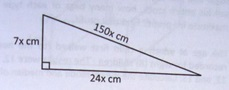
\includegraphics[width=5cm]{./img/quad1.jpg}
	\end{center}
	
	\begin{itemize}
	\item[(i)] Find the value of x
	\item[(ii)] Calculate the area of the triangle
	\end{itemize}		
	
	\item Given the right angled triangle below whose sides are measured in centimeters determine:
		\begin{itemize}
		\item[(i)] The value of x
		\item[(ii)] The area of the triangle
		\end{itemize}
		
		\begin{center}
		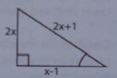
\includegraphics[width=3cm]{./img/quad2.jpg}
		\end{center}
		
	\item Study the following diagram carefully and answer the questions that follow.
	\begin{center}
	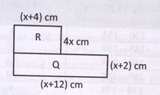
\includegraphics[width=4cm]{./img/quad3.jpg}
	\end{center}	
	
		\begin{itemize}
		\item[(a)]
			\begin{itemize}
			\item[(i)] Write down an expression for the area of rectangle R.
			\item[(ii)] Show that the total area of rectangle R and O is $(5x^2 + 30x + 24)$ cm$^2$.
			\end{itemize}					
		\item[(b)] If the total area of R and Q is 64 cm$^2$, calculate the value of $x$ correct to 1 decimal place.			
		\end{itemize}			

\end{enumerate}
	
	
	
	\subsection{Logarithms}
\begin{enumerate}

	\item Solve $\log_a(x^2 + 3) - \log_ax = 2\log_a2$.
	
	\item Evaluate without using mathematical tables $2\log 5 + \log 36 - \log 9$	
	
	\item Simplify $\cfrac{\log x^4 - \log x}{\log x^3 - \log x}$

	\item Simplify $2\log_{10} 25 - 3\log_{10} 5 + \log_{10} 20$.
	
	\item If $\log_a x = 7$, what is $\log_a \left(\cfrac{1}{x}\right)$?
	
	\item Find the value of the expression $2\log 40 + \log \sqrt{81} - 2\log 12$.
	
	\item Solve for $m$: $\log m = 3\log 6 - \frac{1}{3}\log 125 - 4\log 3 - \log \frac{16}{3}$

	\item Express as a single logarithm the expression $\frac{1}{2}\log_c x - 7\log_c y + \log_c z$.
	
	\item Without using tables, find the value of $3\log_{10} 5 + 5\log_{10} 2 - \frac{1}{2}\log_{10} 16$.
	
	\item Evaluate: $\log_3 9 \times \log_4 \cfrac{1}{64} \times \log_7 \cfrac{1}{7}$
	
	\item Simplify $\log_2 32 - \log_3 9$.
	
	\item It is given that $\log_{10} x + \log_{10} 20 = 2$. Find the value of $x$.
	
	\item Solve the equation $\log_4 5x - \log_4 (x + 2) - \log_4 3 = 0$.
	
	\item Evaluate without using tables $\log_5 \sqrt[3]{605}$
	
	\item If $\cfrac{\log k}{\log 9} = \cfrac{\log 256}{\log 16}$, find the value of $k$.
	
	\item Solve for $x$ in the logarithmic equation $2\log x = \log 4 + \log (2x - 3)$
	
	\item It is given that $n\log_5 125 = \log_2 64$. What is $n$?
	
	\item Find $x$ if $\log_x 32 = 5$.
	
	\item Solve for $x$ if $\log_{10} (x^2 - 3x - 44) = 1$
	
	\item If $\log_4 x = y$, show that $\log_2 x = 2y$. Hence find the value of $x$ given that $\log_2 x + \log_4 x = 9$.
	
	\item Find the value of $a$ if $\log_a 81 - \log_2 32 = -1$.
	
	\item Solve for $x$, given that $\log_3 x - \log_3 (x - 8) = 2$.
	
	\item Without using tables, calculate the value of\\
	(a) $\log_{10}6$	(b) $\log_{10}0.9$\\
	($\log_{10}2 = 0.3010$, $\log_{10}3 = 0.4771$)
	
	\item If $\log 2 = 0.3010$, find the value of $\log 5$.
	
	\item If $\log p = 1.813$ and $\log q = 2.513$, find the value of $pq^2$
	
	\item Using properties of logarithms show that $\log_{10} 15 = 1.17609$ given that $\log_{10} 2 = 0.30103$ and $\log_{10} 3 = 0.47712$.
	
	\item If $\log a = 1.3010$, $\log b = 1.4771$ and $\log c = 1.7782$, calculate $\log \sqrt{\cfrac{a^2b}{c^2}}$ 
	
	\item Evaluate $\log_{10} \cfrac{(0.1575 \times 27500)}{315}$ given that $\log_{10} 1.575 = 0.1973$, $\log_{10} 2.75 = 0.4393$ and $\log_{10} 3.15 = 0.4983$.

	\item Use logarithms to calculate $(3.25)^{10} + \left(\cfrac{40.9}{6.692}\right)^3$\\
	Express your answer in the form $A \times 10^n$, where $1 \leq A < 10$ and $n$ is an integer, to 2 significant figures.
	
	\item By using logarithm tables evaluate: $\sqrt{\cfrac{86.21 \times 2.734}{5.218 \times 0.724}}$
	
	\item Use common logarithm tables to find the value of $\cfrac{2.055 \times 20.35 \times 6.325}{100.5 \times 0.045}$
	
	\item By using logarithm tables evaluate: $\cfrac{88.76 \times 0.0278}{5678 \times 875.8}$

\end{enumerate}


	\subsection{Similarity / Congruence}
\begin{enumerate}

	\item In the figure drawn below find the value of $x$ if $\hat{B} = 37^\circ$.
	
	\begin{center}
	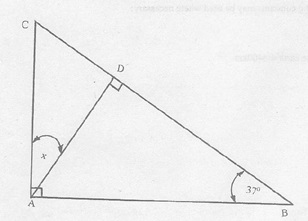
\includegraphics[width=5cm]{./img/sim1.jpg}
	\end{center}
	
	\item In the figure below DE is parallel to BC, AD = 6 cm, BD = 3 cm, DE = 4 cm and $A\hat{B}C = 90^\circ$.
	
	\begin{center}
	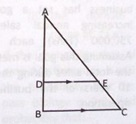
\includegraphics[width=3cm]{./img/sim2.jpg}
	\end{center}
	
	Calculate:
	\begin{itemize}
	\item[(i)] the length of BC
	\item[(ii)] the ratio AE\slash AC
	\end{itemize}
	
	\item In $\bigtriangleup ABC$, $M$ is the midpoint of $\overline{AB}$ and $N$ is the midpoint of $\overline{AC}$. Prove that $\overline{MN} \parallel \overline{BC}$ and $\overline{MN} = \frac{1}{2}\overline{BC}$.
	
	\item The ratio of the area of two similar triangles is 1 : 4. Find the ratio of their corresponding sides.
	
	\item If polygons $X$ and $Y$ are similar and their areas are 16 cm$^2$ and 49 cm$^2$ respectively, what is the length of a side of polygon $Y$ if the corresponding side of polygon $X$ is 28 cm?
	
	\item Triangles O and P are similar. A side of triangle O is 8 cm long, while the corresponding side of triangle P is 16 cm long. If the area of triangle O is 40 cm$^2$, what is the area of triangle P?
	
	\item 
		\begin{itemize}
		\item[(i)] Show whether triangles PQR and ABC are similar or not.
	\begin{center}
	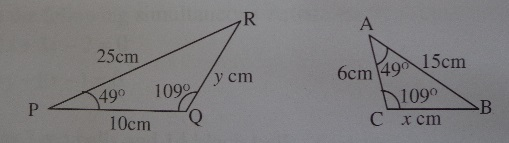
\includegraphics[width=7cm]{./img/sim14.jpg}
	\end{center}
		\item[(ii)] Find the relationship between $y$ and $x$ in the triangles given above.
		\end{itemize}
		
	\item In the figure below, SR is parallel to PQ, SX = 3 cm, XQ = 8 cm, PQ = 12 cm and XR = 2.7 cm.
	\begin{center}
	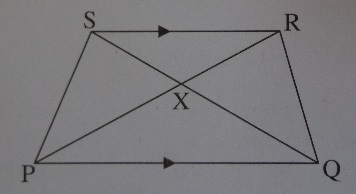
\includegraphics[width=4cm]{./img/sim15.jpg}
	\end{center}
		\begin{itemize}
		\item[(i)] Show that $\bigtriangleup PQX$ and $\bigtriangleup RSX$ are similar.
		\item[(ii)] Calculate the length of SR and PX.
		\end{itemize}
	
	\item With reference to the figure below, calculate the length of segment $\overline{CE}$.
	
	\begin{center}
	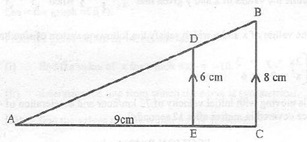
\includegraphics[width=5cm]{./img/sim3.jpg}
	\end{center}

		\item In the figure below, calculate the length $\overline{BC}$ if $\overline{AD} = 4$ cm, $\overline{DE} = 3$ cm, $\overline{CE} = 5$ cm and $A\hat{B}C$ and $A\hat{D}E$ are both right angles.
	
	\begin{center}
	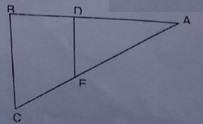
\includegraphics[width=4cm]{./img/sim10.jpg}
	\end{center}

	\item In the figure below, BC is parallel to DE, AB = AC and CE = 2.5 cm. DE = 6 cm. The height of trapezium BCED is 1.5 cm.
	
	\begin{center}
	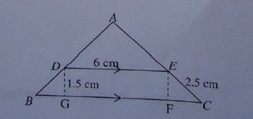
\includegraphics[width=5cm]{./img/sim4.jpg}
	\end{center}

	\begin{itemize}
	\item[(a)] Prove that the triangles ABC and ADE are similar.
	\item[(b)] Calculate the length of AE.
	\end{itemize}
	
	\item In the diagram below, show that $\cfrac{AD}{AB} = \cfrac{CD}{AC}$
	
	\begin{center}
	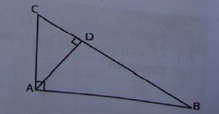
\includegraphics[width=5cm]{./img/sim7.jpg}
	\end{center}

	\item $\bigtriangleup ABC$ is similar to $\bigtriangleup DEF$. AB = 8 cm while DE = 12 cm. Find the area of $\bigtriangleup ABC$ if that of $\bigtriangleup DEF$ is 45 cm$^2$.
	
	\item In the figure below, $\overline{PQ} \parallel \overline{BC}$, $\overline{AP} = 3$ cm, $\overline{AQ} = 2$ cm and the area of $\bigtriangleup APQ = 8$ cm$^2$.
	\begin{center}
	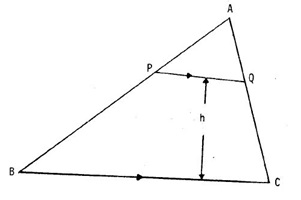
\includegraphics[width=5cm]{./img/sim8.jpg}
	\end{center}

	\begin{itemize}
	\item[(a)] Show that $\bigtriangleup APQ$ is similar to $\bigtriangleup ABC$
	\item[(b)] Find the area of $\bigtriangleup ABC$
	\item[(c)] Calculate the length of (i) $\overline{PQ}$  \quad (ii) $\overline{QC}$ 
	\item[(d)] Calculate the height $h$.
	\end{itemize}
	
	\item In the figure below, $m(A\hat{B}C) = 90^\circ$. Point D on $\overline{BC}$ is such that $\overline{AD}$ bisects $B\hat{A}C$. If AD = 4 cm and $m(A\hat{D}B) = 60^\circ$, calculate the length of:
		\begin{itemize}
		\item[(a)] $\overline{AB}$
		\item[(b)] $\overline{DC}$
		\end{itemize}
		
	\begin{center}
	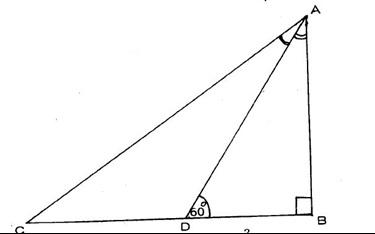
\includegraphics[width=6cm]{./img/sim9.jpg}
	\end{center}
	
	\item In the figure below, $\bigtriangleup ABC$ is similar to $\bigtriangleup CTU$, with AB = 3 cm and CT = 2 cm. The area of $\bigtriangleup CTU$ is 6 square cm. Find the area of $\bigtriangleup ABC$.
	
	\begin{center}
	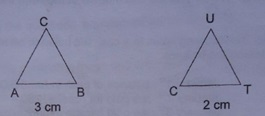
\includegraphics[width=5cm]{./img/sim11.jpg}
	\end{center}
	
	\item PXQ and RXS are straight lines and PR is parallel to SQ. Calculate PX and RX if PR = XQ = 18 cm, XS = 9 cm and SQ = 12 cm.
	
	\begin{center}
	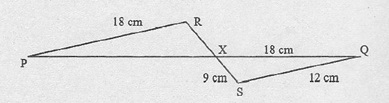
\includegraphics[width=7cm]{./img/sim12.jpg}
	\end{center}	
	
	\item In the figure below, ABCD is a square. If $\overline{AR} = \overline{BR}$ prove that R is the midpoint of $\overline{DC}$.
	
	\begin{center}
	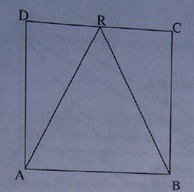
\includegraphics[width=3cm]{./img/sim13.jpg}
	\end{center}	
	
	
%congruency	
	\item ABCD is part of a regular polygon. Show that the triangles ABC and BCD are congruent.
	
	\begin{center}
	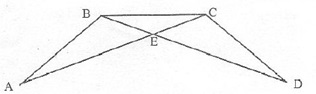
\includegraphics[width=5cm]{./img/sim5.jpg}
	\end{center}
	
	\item In the figure below, $\overline{AC} = \overline{CB}$ and $D\hat{A}C$ and $D\hat{B}C$ are right angles. Prove that $\bigtriangleup ACD \equiv \bigtriangleup CBD$.
	
	\begin{center}
	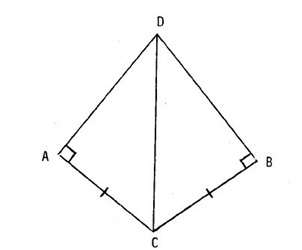
\includegraphics[width=5cm]{./img/sim6.jpg}
	\end{center}
	
\end{enumerate}	

	\subsection{Geometrical Transformations}
	
	See Form IV \nameref{f4trans}.

	\subsection{Pythagoras Theorem}
	
	See \nameref{f2quadeqnsgeo} in Form II \nameref{f2quadeqns} as well as applications in Form IV \nameref{f4trig}.
	
	\subsection{Trigonometry}
	
	See Form IV \nameref{f4trig}.
	
	\subsection{Sets}
\begin{enumerate}

	\item A survey conducted at Omega secondary school showed that 15 students play volleyball, 11 play basketball and 6 play both volleyball and basketball. If everyone plays at least one of these games, find the number of students who play the following games (using a Venn diagram):
		\begin{itemize}
		\item[(a)] volleyball or basketball;
		\item[(b)] basketball but not volleyball;
		\item[(c)] volleyball only.
		\end{itemize}

	\item In a class of 30 students, 17 participate in English debate, 12 participate in English debate and sports. If every student is required to participate in at least one of these two events, find the number of students who participate in:
	\begin{itemize}
	\item[(i)] English debate only
	\item[(ii)] sports only.
	\end{itemize}

	\item In a class of 42 students, 31 students study History and 26 study Physics. Using VVenn diagrams or otherwise, find the number of students who study Physics only.
	
	\item In a certain school there are 50 pupils studying both Basic Mathematics and Additional Mathematics. School regulations require that an Additional Mathematics pupil must come from the Basic Mathematics class. In the school, 10 pupils do not study Basic Mathematics. If only 100 pupils study Basic Mathematics but not Additional Mathematics, how many pupils:
	\begin{itemize}
	\item[(i)] are in the school?
	\item[(ii)] study either Basic Mathematics or Additional Mathematics?
	\item[(iii)] do not study Additional Mathematics?
	\end{itemize}
	\noindent Hint: (Use Venn diagram)
	
	\item There are 60 people at a meeting. 35 are businesspersons, 32 are employees and 15 are both businesspersons and employees.
	\begin{itemize}
	\item[(i)] How many are businesspersons or employees?
	\item[(ii)] How many are neither businesspersons nor employees?
	\end{itemize}
	
	\item There are 30 men at a wedding. Twenty are businessmen, twelve are fishermen and 6 are both businessmen and fishermen.
	\begin{itemize}
	\item[(i)] How many are neither businessmen nor fishermen?
	\item[(ii)] How many are either businessmen or fishermen?
	\end{itemize}
	
	\item 
	\begin{itemize}
	\item[(a)] In a boys' school of 200 students, 90 play football, 70 play basketball and 50 play tennis; 26 play basketball and football, 20 play basketball and tennis, 16 play tennis and football while 10 play all three games. Represent this information in a well labeled Venn diagram.
	\item[(b)] From the information given in (a), how many students in the school do not play:
	\begin{itemize}
	\item[(i)] football
	\item[(ii)] basketball
	\item[(iii)] tennis.
	\end{itemize}
	\end{itemize}
	
	\item Student test results on three subjects; Mathematics, Physics and Chemistry show that 20 passed Chemistry, 5 passed all three subjects, 12 passed Mathematics and Physics and 16 passed Mathematics and Chemistry. Each student passed at least two subjects.
	\begin{itemize}
	\item[(i)] Draw a well labeled Venn diagram to represent these results.
	\item[(ii)] How many students passed Physics and Chemistry?
	\item[(iii)] How many students did the test?
	\end{itemize}

	\item A survey of 240 houses showed that all of them kept a farm or a garden or both. If 180 kept gardens and 79 kept farms, how many houses kept both?
	
	\item In a school of 75 pupils, 45\% of the pupils take Biology but not Chemistry, 32\% take both subjects and 10\% of them take Chemistry but not Biology. How many pupils do not take either Biology or Chemistry?
	
	\item In a Form four class of 24 students, 10 students take basic mathematics only, 12 students take physics and 4 students take both subjects. Using a Venn diagram, find:
	\begin{itemize}
	\item[(i)] The number of students taking physics only.
	\item[(ii)] The number of students taking mathematics.
	\item[(iii)] The number of students who take neither of the two subjects
	\end{itemize}
	
	\item In a class of 36 students, 24 take Chemistry whilst 17 take Physics. What is the least possible number of students who must be taking both Physics and Chemistry?
	
	
%not word problems	
	\item $A$ and $B$ are subsets of the universal set $U$. Find n$(A \cap B)$ given that n$(A) = 39$, n$(A' \cap B') = 4$, n$(B') = 24$ and n$(U) = 65$.

	\item Given $A = \{(x,y):3x + 4y = 10\}$ and $B = \{(x,y):2x - 3y = 1\}$, find $A \cap B$.
	
	\item If $\mu = \{x:1 < x < 11\}$, $A = \{x:2 < x \leq 9\}$, $B = \{x:2 \leq x < 10\}$, list the elements belonging to:
	\begin{itemize}
	\item[(i)] $A \cup B$
	\item[(ii)] $A' \cap B$
	\end{itemize}
	
	\item $P$ and $Q$ are finite sets such that n$(P \cap Q') = 15$, n$(P \cup Q) = 90$ and n$(P \cap Q) = 30$. Without using a Venn diagram, find n$(Q)$.
	
	\item If $A = \{a, b, c\}$, $B = \{b, c, d\}$ and $C = \{c, d, e\}$, show that $A \cup (B \cap C) = (A \cup B) \cap (A \cup C)$.
	
	\item If $\xi = \{a, b, c, d, e\}$, $A = \{a, b, c\}$ and $B = \{e, d\}$, find:
		\begin{itemize}
		\item[(i)] $A' \cap B'$
		\item[(ii)] $(A \cap B)'$
		\end{itemize}
		
	\item If n$(A) = 8$, n$(B) = 12$ and $(A \cap B) = 5$, find n$(A \cup B)$.
		
	\item If $\mu = \{p, q, r, s\}$, If $A = \{p, q, r\}$ and If $B = \{r, s\}$, find $(A' \cap B')$.
		
	\item If $A$ and $B$ are subsets of $S$ where\\
	$S = \{x: x$ is a natural number less than 20$\}$\\
	$A = \{x: x$ is an even number$\}$\\
	$B = \{x: x$ is a multiple of 3$\}$\\
	Find: (a) n$(A \cap B)$ \quad (b) n$(A' \cup B')$
	
	\item If $A$ is the set of prime factors of 42 and $B$ is the set of prime factors of 330, find n$(A \cap B)$.
	
	\item Given sets $A = \{x:-5 \leq x < 2\}$ and $B = \{x:-1 < x < 4\}$, find the value of $A \cap B$.
	
	\item Given $N = \{x:1 \leq x \leq 20\}$. Find the following subsets of $N$:
		\begin{itemize}
		\item[(i)] $A = \{x: x$ is a multiple of 3$\}$
		\item[(ii)] $B = \{x: x$ is a multiple of 4$\}$
		\item[(iii)] $A'$ \quad (iv) $B'$ \quad (v) $(A \cup B)'$ \quad and \quad (vi) $A' \cap B'$.
		\end{itemize}
		
	\item If $A$ and $B$ are any two disjoint sets, show the region represented by $A' \cap B'$ on a Venn diagram.
	
	\item $U = \{10, 20, 30, 40\}$, $A = \{10, 30\}$, $B = \{40, 10\}$, find:
		\begin{itemize}
		\item[(a)]
			\begin{itemize}
			\item[(i)] $A' \cup B'$
			\item[(ii)] $A \cap B'$
			\end{itemize}
		\item[(b)] If $A$ is a subset of $B$, represent the two sets in a Venn diagram.
		\end{itemize}
		
	\item If n$(A \cap B') = 8$, n$(B \cap A') = 5$ and n$(A \cup B) = 20$, 
		\begin{itemize}
		\item[(i)] Display the information in a Venn diagram.
		\item[(ii)] Give the values of n$(A)$ and n$(B)$.
		\end{itemize}
		
	\item Given that $A = \{x:0 \leq x \leq 8\}$ and $B = \{x:3 \leq x \leq 11\}$, where $x$ is an integer, in the same form, present in a Venn diagram:\\
	(i) $A \cup B$ \quad (ii) $A \cap B$\\
	and hence find the elements in each set.
	
	\item If $E = \{$integers between 1 and 11$\}$\\
	$A = \{x:2 < x \leq 9\}$\\
	$B = \{x:1 \leq x < 10\}$
		\begin{itemize}
		\item[(a)] Draw a Venn diagram to illustrate these sets.
		\item[(b)] List the elements belonging to:\\
			(i) $A \cup B$ \quad (ii) $A' \cap B$
		\item[(c)] State n$(A \cap B')$
		\end{itemize}
		
	\item From the figure below, answer the following questions.
	
	\begin{center}
	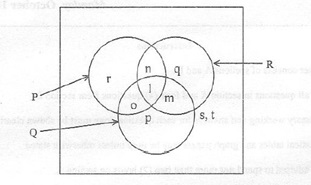
\includegraphics[width=6cm]{./img/set1.jpg}
	\end{center}
	
	\begin{itemize}
	\item[(a)] List down members of $(P \cup Q)'$
	\item[(b)] Find n$(P \cup Q \cup R)'$
	\item[(c)] Find n$(Q \cup R) - $ n$(P \cap R)$
	\end{itemize}
	
	\item In the Venn diagram below, the number of elements in various regions are as indicated.\\
	If n$(A \cup B \cup C) = 150$, find the value of $x$.
	
	\begin{center}
	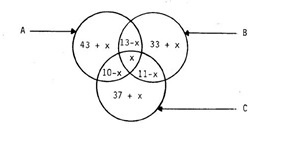
\includegraphics[width=7cm]{./img/set2.jpg}
	\end{center}
	
	\item In the figure drawn below, find the number of elements in sets:
		\begin{itemize}
		\item[(a)] $A' \cap (B \cup C)$
		\item[(b)] $(A' \cap B') \cup (B \cup C')$
		\end{itemize}
		
	\begin{center}
	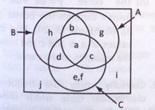
\includegraphics[width=5cm]{./img/set3.jpg}
	\end{center}
	

\end{enumerate}


	\subsection{Statistics}
	
	See Form III \nameref{f3stats}.


\section{Form III}

	\subsection{Relations / Functions}
\begin{enumerate}


			\subsubsection{Graphs, Domain, Range}
%relations

	\item Consider the relation $R = \{(x,y): y = x^2 + 4x\}$
		\begin{itemize}
		\item[(a)] Complete the following table for the relation $R$.\\
		\begin{tabular}{|c|c|c|c|c|c|c|c|c|c|c|} \hline
		$x$ &-6&-5&-4&-3&-2&-1&0&1&2&3 \\ \hline
		$y$ &&&&&&&&&& \\ \hline
		\end{tabular}
		\item[(b)] Plot the graph of the relation $R$.
		\item[(c)] Use the graph to solve the equation $x^2 + 3 = -4x$.
		\end{itemize}
		
	

		
%functions
	\item A function $f$ is defined by $f: \rightarrow 2x^2 - 2x - 1$ where $x$ is the set $\{-2, -1, 0, 1, 2, 3\}$;
		\begin{itemize}
		\item[(a)] Write down the set of ordered pairs $(x, f(x))$.
		\item[(b)] Represent the set of ordered pairs $(x, f(x))$ in a pictorial diagram.
		\item[(c)] Draw the graph of $f(x)$.
		\item[(d)] Find the maximum or minimum value of the function $f(x) = 2x^2 - 2x - 1$.
		\end{itemize}

	\item A function $f$ is defined by the formula $f(x) = \sqrt{x}$, where $x$ is a whole number.
		\begin{itemize}
		\item[(a)] Evaluate $f(9)$
		\item[(b)] If $f(x) = 16$, find the value of $x$.
		\item[(c)] Find the value of $\cfrac{f(200)}{f(2)}$
		\end{itemize}		
		
	\item A function $f$ is defined by: $f(x) = |x - 2|$.
		\begin{itemize}
		\item[(i)] Evaluate $f(-3)$.
		\item[(ii)] Find $x$ if $f(x) = 6$.
		\end{itemize}		 
		
	\item If $f(x) = 5x^2 + 17x - 12$,
		\begin{itemize}
		\item[(a)]
			\begin{itemize}
			\item[(i)] Evaluate $f(10) - f(5)$
			\item[(ii)] Factorize $f(x)$
			\end{itemize}
		\item[(b)] Determine the domain and range of $f(x)$
		\end{itemize}
		
	\item The curve $y = ax^2 + bx + c$ passes through the points (1,8), (0,5) and (3,20). Find the values of $a$, $b$ and $c$ and hence the equation of the curve.
	
	\item If $f(x) = \cfrac{x + 2}{x^2 - x- 6}$, find the values of $x$ for which the function is not defined.
	
	\item The function $f$ is defined by $f: \rightarrow ax + b$, for $x \in R$, where $a$ and $b$ are constants. It is given that $f(2) = 1$ and $f(5) = 7$.
		\begin{itemize}
		\item[(i)] Find the value of $a$ and $b$
		\item[(ii)] Solve the equation $f \circ f(x) = 0$
		\end{itemize}
		
	\item Draw the graph of $x^2 = 2 + y$.
	
	\item It has been specified that $f(x) = 2x^2 - 5x - 3$ ranges from $x = -2$ to $x = 4$.
		\begin{itemize}
		\item[(a)] Draw the graph of $f(x)$.
		\item[(b)] From the graph drawn in (a) above:
			\begin{itemize}
			\item[(i)] find the value of $x$ for which $f(x) = -10$.
			\item[(ii)] determine the line from which the curve is symmetrical.
			\item[(iii)] find the values of $x$ by which $f(x)$ is negative.
			\item[(iv)] solve the equation $2x^2 - 5x - 3 = 0$.
			\end{itemize}
		\end{itemize}

	\item A function is defined by $f(x) = \cfrac{x}{x + 3}$; sketch the graph of $f$.
	
	\item 
		\begin{itemize}
		\item[(a)] On the same set of axes draw the graphs of $f(x) = x^2 - 4x$ and $y = x - 2$.
		\item[(b)] Using the two graphs in (a), estimate the values of $x$ for which $x^2 - 5x + 2 = 0$, correct to 2 significant digits.
		\end{itemize}
		
		\item Without using a table of values, draw the graph of $y = -x^2 + 4x - 5$ and use it to solve the equation $-x^2 + 4x - 5 = -10$.
		
		\item Sketch the graph of the function $f(x) = -1 + |x|$ and find:
			\begin{itemize}
			\item[(i)] the domain and \quad (ii) the range, of $f(x)$.
			\end{itemize}
			
	\item Sketch the graph of the rational function $y = \cfrac{3x - 4}{x - 3}$ and determine its range.
	
	\item 
		\begin{itemize}
		\item[(a)] 
			\begin{itemize}
			\item[(i)] Draw the graphs of the functions $f(x) = x^2 - 4$ and $g(x) = x + 2$ in the same coordinate system.
			\item[(ii)] Shade the region enclosed by the graphs in (i) indicating the intercepts for both graphs.
			\end{itemize}
		\item[(b)] From the graphs in (a) write the coordinates of the points where $f(x) = g(x)$.
		\item[(c)] State the domain and range of $f(x)$.
		\end{itemize}
		
	\item The functions $f$ and $g$ are defined for the domain: $\{2, 3, 4, 5, 6\}$ and the range of $f = \{8, 10, 12, 14, 16\}$ and that of $g = \{8, 6, 4, 2, 0\}$. Find $fg(3)$.
	
	\item Find the domain and range of $f(x) = \sqrt{1 - x^2}$.
	
	\item Find the domain and range of the relation $y = 3x^2 + 2$.
	
	\item Compute the range of the function $f(x) = x^2 - 4x + 3$ for which the domain is $\{-2, -1, 0, 1, 2, 3\}$.
	
	\item Given the rational function $g(x) = \cfrac{mx^2}{x^2 - 3x + 2}$, determine its domain and range.
	
	\item If $f$ is a function such that:\\
	$f(x) =
	\begin{cases}
	\-3 & \text{if } x \leq -1 \\
	1 & \text{if } -1 < x \leq 2 \\
	4 & \text{if } 2 < x
	\end{cases}$
	
	\begin{itemize}
	\item[(a)] determine the domain and range of $f(x)$.
	\item[(b)] draw the graph of $f(x)$.
	\end{itemize}
	
			\subsubsection{Inverse Functions}
%inverses	
	\item Write down the inverse of the function $f(x) = \frac{1}{2}x + 5$.
	
	\item If $f(x) = \frac{1}{2}x + 5$, find $f^{-1}(6)$.
	
	\item A function is defined by $f(x) = x^2 - 2$. Find:
		\begin{itemize}
		\item[(i)] the inverse, $f^{-1}(x)$ of this function.
		\item[(b)] the value of $f^{-1}(-2)$.
		\item[(c)] the domain of $f^{-1}(x)$.
		\end{itemize}
		
	\item Find $g^{-1}(x)$ and hence evaluate $g^{-1}(18)$ given that $g(x) = 2^x + 2$.
	
	\item Find the inverse of the relation $y = \cfrac{4x + 1}{x - 2}$.
	
	\item Find the inverses of the following:
		\begin{itemize}
		\item[(a)] $\{R = (x,y): y = 4x^2\}$
		\item[(b)] $f(x) = 20^x$
		\end{itemize}
		
	\item The functions $f$ and $g$ are defined by: $f(x) = |x|$ and $g(x) = 2 - 3x$.
		\begin{itemize}
		\item[(i)] Evaluate $f(-3)$.
		\item[(ii)] Find $g^{-1}(x)$ and hence evaluate $g^{-1}(8)$.
		\item[(iii)] Draw on the same axes the graphs of $f$ and $g$.
		\end{itemize}

	\item 
		\begin{itemize}
		\item[(a)] If $f(x) = -2x + 3$ find $f^{-1}(3)$.
		\item[(b)] Draw the graph of $f(x) = |x - 1|$ for $-4 \leq x \leq 4$
		\item[(c)] State the domain and range of $f(x) = |x - 1|$.
		\end{itemize}
		
	\item If $f(x) = x^2 - 4x + 3$, find\\
	(i) $f^{-1}(x)$ \quad (ii) the domain and range of $f(x)$
	
	\item A function is defined by $f(x) = x^2 + 6$ and $g(x)$ is another function of $x$ such that\\
	 $g(x) = \cfrac{f(x) - f(4)}{x - 4}$. \\
	Find (i) $g(-4)$ \quad (ii) $g^{-1}(5)$
	
	\item Given that $g(x) = 5 + \cfrac{x}{2}$, find the values of:\\
	(i) $g^{-1}(6)$ \quad (iii) $g^{-1}(-1)$\\
	(ii) $g^{-1}(0)$ \quad (iv) $g^{-1}(a)$
	
			\subsubsection{Maximum, Minimum Values}
%max, min value	
	\item Find the maximum value of the quadratic equation $2 + 30t - 5t^2$.
	
	\item Draw a graph of the function $y = x^2 - 3x + 2$ for the values of $x$ from -2 to 5. From your graph, find:
		\begin{itemize}
		\item[(a)] the range of the function.
		\item[(b)] the minimum value of $y$ and the value of $x$ at which this minimum value occurs.
		\item[(c)] the solution of the equation $x^2 - 3x - 4 = 0$.
		\item[(d)] the solution of the inequality $x^2 - 3x + 2 > 0$.
		\end{itemize}
		


\end{enumerate}	
	
	
	
	
	\subsection{Statistics} \label{f3stats}
\begin{enumerate}

	\item The table below show the distribution of the ages of boys in one class at Shivone secondary school.\\
	\begin{tabular}{|l|c|c|c|c|} \hline
	Age in years & 14 - 16&17 - 19&20 - 22&23 - 25\\ \hline
	Number of boys&27&14&8&7\\ \hline	
	\end{tabular}
		\begin{itemize}
		\item[(a)] Draw a cumulative frequency polygon for this information.
		\item[(b)] What is the mean age of the class?
		\item[(c)] State the median class.
		\item[(d)] Find the probability that a boy chosen at random from the class has age between 17 - 19 or 23 - 25.
		\end{itemize}

	\item In a survey of the number of children in 12 houses, the following data resulted: 1, 2, 3, 4, 2, 2, 1, 3, 4, 3, 5, 3.
		\begin{itemize}
		\item[(a)] Show this data in a frequency distribution table.
		\item[(b)] Draw a histogram and a frequency polygon to represent this data.
		\item[(c)] Calculate the mean and mode number of children per house.
		\end{itemize}

	\item The following is a record of marks by a group of students in an examination.\\
	
	\begin{tabular}{cccccccccc}
	23&63&82&71&12&63&38&17&23&44 \\
	54&19&70&45&70&43&18&03&02&64 \\
	45&42&40&70&63&28&18&27&58&53 \\
	23&81&70&58&31&83&19&43&72&71 \\
	48&63&62&44&38&37&46&81&73&38 	
	\end{tabular}
	
	\begin{itemize}
	\item[(a)] Tabulate as a frequency distribution using intervals 0 - 9, 10 - 19, etc.
	\item[(b)] Find the class which contains the median.
	\item[(c)] Find the modal class.
	\item[(d)] Calculate the mean mark using the grouped data.
	\end{itemize}
	
	\item The following frequency distribution table shows the monthly salaries for 33 workers in a certain company.\\
	
	\begin{tabular}{|p{2.5cm}|c|c|c|c|c|} \hline
	\textbf{Salary (Tsh)}&20000 - 29000&30000 - 39000&40000 - 49000&50000 - 59000&60000 - 69000 \\ \hline
	\textbf{Number of Workers}&1&4&6&10&8 \\\hline
	\end{tabular}

	\begin{tabular}{|p{2.5cm}|c|c|} \hline
	\textbf{Salary (Tsh)}&70000 - 79000&80000 - 89000 \\ \hline
	\textbf{Number of Workers}&2&2 \\\hline
	\end{tabular}
	
	\begin{itemize}
	\item[(a)] By making the class mark of the class interval 50000 - 59000 as the assumed mean, calculate the mean salary.
	\item[(b)] What is the mode for this distribution?
	\item[(c)] Calculate the median.
	\item[(d)] Find the number of workers whose salaries exceed Tsh 69,500/=.
	\end{itemize}
	
	\item The following table gives the scores of sixty students in a Basic Mathematics test.\\
	
	\begin{tabular}{|c|c|} \hline
	Scores&Frequency \\ \hline
	0 - 10&5 \\ \hline
	10 - 20&7 \\ \hline
	20 - 30&15 \\ \hline
	30 - 40&25 \\ \hline
	40 - 50&8 \\ \hline
	\end{tabular}
	
	Calculate:
	\begin{itemize}
	\item[(a)] The mean score if the assumed mean is obtained from the mid mark of the modal class.
	\item[(b)] The median.
	\item[(c)] The range.
	\end{itemize}
	
	\item Carefully study the frequency distribution table which shows marks for 40 students in a mathematics examination.\\
	
	\begin{tabular}{|l|c|c|c|c|c|} \hline
	Marks & 1 - 20&21 - 40&41 - 60&61 - 80&81 - 100\\ \hline
	Number of Students&3&11&12&8&6\\ \hline	
	\end{tabular}
	
	\begin{itemize}
	\item[(i)] Calculate the mean score, given the assumed mean 50.5.
	\item[(ii)] Determine the modal class.
	\item[(iii)] Draw a cumulative frequency curve and use it to estimate the median.
	\end{itemize}
	
	\item A survey of 50 families showed the number of children per family as follows.\\
	
	\begin{tabular}{|l|c|c|c|c|c|} \hline
	Number of children&1&2&3&4&5 \\ \hline
	Number of families&19&18&9&3&1 \\ \hline	
	\end{tabular}
	
	\begin{itemize}
	\item[(i)] Write down the modal number of children per family.
	\item[(ii)] Find the median number of children per family.
	\item[(iii)] Calculate the mean number of children per family.
	\end{itemize}
	
	\item The age at which a child first walked (to the nearest month) was recorded for eight (8) children. The results were 12, 10, 16, 19, 10, 12, 12 and 13. Calculate the mean, mode and median of the data.
	
	\item A random sample of 100 students was chosen from a school. Each student's blood pressure was measured to the nearest milimetres of mercury as shown in the table below.\\
	
	\begin{tabular}{|l|c|c|c|c|c|c|c|} \hline
	Blood pressure (mmHg)&55 - 59&60 - 64&65 - 69&70 - 74&75 - 79&80 - 84&85 - 89 \\ \hline
	Number of students&1&3&8&17&30&25&16 \\ \hline
	\end{tabular}
	
	\begin{itemize}
	\item[(a)] Calculate the mean and mode of blood pressure.
	\item[(b)] Construct a cumulative frequency table and draw the ogive. From the ogive estimate
		\begin{itemize}
		\item[(i)] the median blood pressure
		\item[(ii)] the percentage of students with blood pressure between 67 mmHg and 76 mmHg.
		\end{itemize}
	\end{itemize}
	
	\item Carefully study the frequency distribution table for the scores of 68 students (in percentage) given here under.\\
	
	\begin{tabular}{|p{3cm}|c|c|c|c|c|c|c|} \hline
	Class Boundary (in percentage)&30 - 39&40 - 49&50 - 59&60 - 69&70 - 79&80 - 89&90 - 99 \\ \hline	
	Frequency&6&12&14&16&8&6&6 \\ \hline
	\end{tabular}
	
	\begin{itemize}
	\item[(a)] Determine the mode of the scores.
	\item[(b)] Calculate the median of the scores.
	\item[(c)] A student is chosen at random from the frequency distribution table above. What is the probability that his score is below 60\%?
	\end{itemize}
	
	\item A survey was made on the number of the people attending conferences on one particular week. A random sample of 100 conference centres was taken and the results were as follows:\\
	
	\begin{tabular}{|c|c|} \hline
	\textbf{Number of people}& \textbf{Number of}\\ 	\textbf{attending conference}&\textbf{conference centres} \\ \hline
	150 - 154&8 \\ \hline
	155 - 159&16 \\ \hline
	160 - 164&43 \\ \hline
	165 - 169&29 \\ \hline
	170 - 174&4 \\ \hline	
	\end{tabular}
	
	\begin{itemize}
	\item[(i)] Draw a histogram and a cumulative frequency curve to represent these results.
	\item[(ii)] Estimate the median of this data from the cumulative frequency curve in (i) above.
	\end{itemize}
	
	\item The pie chart below shows the number of students in one examination centre in different subjects sat for the national examinations.
	
	\begin{center}
	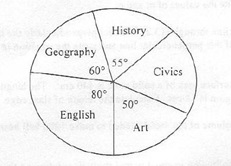
\includegraphics[width=5cm]{./img/stats1.jpg}
	\end{center}
%	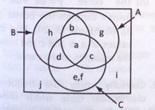
\includegraphics[width=5cm]{./img/set3.jpg}
%	\end{center}	
	
	Given that 220 candidates did History, find:
	\begin{itemize}
	\item[(i)] The total number of candidates at this examination centre.
	\item[(ii)] The number of students who sat for Civics examination.
	\end{itemize}
	
	\item The following represents age distribution of members of a school choir.\\
	
	\begin{tabular}{|l|c|c|c|c|c|c|} \hline
	Age&14&15&16&17&18&19 \\ \hline
	Frequency&2&1&3&6&5&3 \\ \hline	
	\end{tabular}
	
	\begin{itemize}
	\item[(a)] How many students are in the school class?
	\item[(b)] What is the modal age?
	\item[(c)] Calculate the mean age of the members of the school choir.
	\item[(d)] What is the probability that a member chosen at random from the choir is
		\begin{itemize}
		\item[(i)] 17 years old?
		\item[(ii)] over or equal to 17 years?
		\end{itemize}
	\item[(e)] Draw a pie chart to show the age distribution of the members of the school choir.
	\end{itemize}
	
	\item The data below represent masses in kg of 36 men:\\
	51; 61; 60; 70; 75; 71; 75; 70; 74; 73; 72; 82; 70; 71; 76; 74; 50; 68; 68; 66; 65; 72; 69; 64; 83; 63; 83; 58; 80; 90; 50; 89; 55; 62; 62; 61.
	\begin{itemize}
	\item[(i)] Prepare a frequency distribution table of class interval of size 5 beginning with the number 50 taking into consideration that both the lower limit and upper class limit are inclusive.
	\item[(ii)] Calculate the mean and mode from the frequency distribution table prepared in (i) above by using assumed mean from the class mark of the modal class.
	\end{itemize}
	
	\item The data below shows test scores of a certain class in mathematics.
	
	\begin{tabular}{cccccccccc}
	21&21&21&22&22&22&22&23&23&24 \\
	24&24&21&24&24&25&26&27&27&27 \\
	\end{tabular}
	
	Construct a frequency distribution table showing scores $x$ and frequency $f$.
	
	\item Carefully study the frequency distribution table which shows marks for 40 students in a mathematics examination.\\
	
	\begin{tabular}{|l|c|c|c|c|c|} \hline
	Marks & 1 - 20&21 - 40&41 - 60&61 - 80&81 - 100\\ \hline
	Number of Students&3&11&12&8&6\\ \hline	
	\end{tabular}
	Determine:
	\begin{itemize}
	\item[(i)] The mean, given the assumed mean is 50.5
	\item[(ii)] The median
	\item[(iii)] Modal class and its corresponding class mark.
	\end{itemize} 
	
	\item The table shows the masses of 100 students to the nearest kilogram.\\
	
	\begin{tabular}{|l|c|c|c|c|c|} \hline
	Mass (kg) &60 - 62&63 - 65&66 - 68&69 - 71&72 - 74 \\ \hline
	Frequency&5&18&42&27&8 \\ \hline	
	\end{tabular}
	
	\begin{itemize}
	\item[(a)] Determine the mean of the masses.
	\item[(b)] Find the mode.
	\item[(c)] Draw a cumulative frequency curve and use it to determine the median of the masses.
	\end{itemize}
	
	\item The table below shows the distribution of 100 shops and their profit per shop recorded in a certain month.\\
	
	\begin{tabular}{|l|c|c|c|c|c|c|} \hline
	Profit per shop in thousands of shs.&30 - 34&35 - 39&40 - 44&45 - 49&50 - 54&55 - 59 \\ \hline
	Number of shops&12&18&C&C - 7&C - 10&6 \\ \hline	
	\end{tabular}
	
	\begin{itemize}
	\item[(a)] Find the value of C.
	\item[(b)] Prepare the frequency distribution and use it to determine the modal class.
	\item[(c)] Draw a histogram and frequency polygon on the same diagram.
	\end{itemize}
	
	\item The frequency distribution of the length of a sample of 100 nails, measured to the nearest mm, is shown below.\\
	
	\begin{tabular}{|l|c|c|c|c|c|c|c|} \hline
	Length&40 - 42&43 - 45&46 - 48&49 - 51&52 - 54&55 - 57&58 - 60 \\ \hline
	Frequency&4&9&13&20&34&18&2 \\ \hline	
	\end{tabular}
	
	\begin{itemize}
	\item[(a)] How many nails have length less than 51.5 mm?
	\item[(b)] Calculate the mean length.
	\item[(c)] Draw a histogram and use it to estimate the modal length.
	\item[(d)] State the modal class.
	\end{itemize} 
	
	\item The daily wages of one hundred men are distributed as shown below:\\
	
	\begin{tabular}{|p{4cm}|c|c|c|c|} \hline
	Wage in Tshs $\times$ 1000&3.0 - 3.4&3.5 - 3.9&4.0 - 4.4&4.5 - 4.9 \\ \hline
	Number of men&4&6&10&14 \\ \hline	
	\end{tabular}
	
	\begin{tabular}{p{4cm}|c|c|c|c|} \cline{2-5}
	&5.0 - 5.4&5.5 - 5.9&6.0 - 6.4&6.5 - 6.9 \\ \cline{2-5}
	&x&20&14&6 \\ \cline{2-5}	
	\end{tabular}
	
	\begin{itemize}
	\item[(a)] Find x.
	\item[(b)] Calculate the daily mean wage of the 100 men.
	\item[(c)] Draw a histogram to represent this data.
	\end{itemize}
	
	\item The table below shows the distribution of scores of 46 students in a mathematics examination.\\
	
	\begin{tabular}{|l|c|c|c|c|c|} \hline
	Marks in \%&35 - 45&46 - 56&57 - 67&68 - 78&79 - 89 \\ \hline
	No. of students&20&12&7&6&1 \\ \hline	
	\end{tabular}
	
	\begin{itemize}
	\item[(a)] 
		\begin{itemize}
		\item[(i)] Calculate the mean score.
		\item[(ii)] What is the modal class?
		\end{itemize}		 
	\item[(b)] Draw a cumulative frequency curve and estimate from  it the median score.
	\end{itemize} 
	
	\item The heights in centimetres of 100 students of a certain school were recorded as follows:\\
	
	\begin{tabular}{|l|c|c|c|c|c|c|c|c|c|} \hline
	Height in cm&150&155&160&165&170&175&180&185&190 \\ \hline
	Frequency&4&9&12&16&25&20&8&4&2 \\ \hline	
	\end{tabular}
	
	From the above information answer the following questions:
	\begin{itemize}
	\item[(a)] Draw a frequency polygon.
	\item[(b)] Determine the mean, median and mode.
	\item[(c)] Compute the variance and standard deviation.
	\item[(d)] A student is chosen at random from this school. What is the probability that his height is greater than 160 cm?
	\end{itemize} 
	
	\item The following table shows the grade points scored by 50 students in a Mathematics test.\\
	
	\begin{tabular}{|l|c|c|c|c|c|c|} \hline
	Grade points&0&1&2&3&4&5 \\ \hline
	Frequency&1&12&14&15&7&1 \\ \hline	
	\end{tabular}
	
	\begin{itemize}
	\item[(i)] Represent this information by a frequency polygon. 
	\item[(ii)] Find the mode and median.
	\item[(iii)] Find the probability that, if a student is chosen at random, then her grade point score will be greater than or equal to 3.
	\end{itemize} 
	
	\item The examination results (rounded to the nearest whole number \%) are given for a group of students.\\
	
	\begin{tabular}{|l|c|c|c|c|c|} \hline
	Mark (\%)&30 - 39&40 - 49&50 - 59&60 - 69&70 - 79 \\ \hline
	Frequency &5&3&20&2&10 \\ \hline	
	\end{tabular}
	
	\begin{itemize}
	\item[(a)] State the modal class.
	\item[(b)] Estimate the mean score.
	\item[(c)] Estimate the median score.
	\item[(d)] Estimate the mode.
	\end{itemize} 
	
	\item The scores of a Physics test taken by 60 students were recorded as follows:\\
	
	\begin{tabular}{ccccccccccccc}
	30&56&21&49&34&58&22&38&27&31&35&41&53 \\
	25&34&48&33&58&20&34&30&50&26&52&32&63 \\
	25&50&36&29&34&21&61&33&51&20&41&30&57 \\
	26&28&45&36&59&26&60&42&21&63&56&36&54 \\
	43&24&30&27&26&56&35&32&&&&& \\	
	\end{tabular}
	
	\begin{itemize}
	\item[(a)] Arrange these scores into grouped frequency distribution table starting with the classes 20 - 24, 25 - 29, 30 - 34, $\ldots$
	\item[(b)] Calculate the mean score.
	\item[(c)] Draw the histogram and use it to estimate the mode.
	\item[(d)] Draw the ogive and use it to estimate the median.
	\end{itemize}
	
	\item Florina sat for ten examinations. In the first six subjects she scored an average of 65 marks while in the last four subjects she scored an average of 60 marks. Find the average score for all the ten examinations.
	
	\item The mean of $n$ numbers is 20. If the same numbers together with 30 give a new mean of 22, find $n$.
	
	\item Find the geometric mean and arithmetic mean of 18 and 72.
	
	\item Calculate the geometric mean and arithmetic mean of $3 + \sqrt{5}$ and $3 - \sqrt{5}$.
	
	\item The arithmetic mean and geometric mean of two numbers $m$ and $n$ are 17 and 15 respectively. Find the two numbers.
	

\end{enumerate}	
	
	
	
	\subsection{Rates and Variations}
\begin{enumerate}

		\subsubsection{Variations}
%variations
	\item If $y$ is directly proportional to $x$, find the value of each of $a$, $b$ and $c$ in the table below.\\
	\begin{tabular}{|c|c|c|c|c|} \hline
	$y$ & 8 & 12 & $b$ & 32 \\ \hline
	$x$ & 2 & $a$ & 6 & $c$ \\ \hline
	\end{tabular}

	\item $x$ is directly proportional to $y^2$ and inversely proportional to $z$. If $x = 10$ when $y = 2$ and $z = 2$, find $x$ when $y = 6$ and $z = 9$.
	
	\item Given that $p$ varies directly proportional to $q$ but inversely proportional to $r$ and that, when $p = 35$, $q = 7$ and $r = 6$. Find the value of $p$ when $q = 2$ and $r =5$.
	
	\item Given that $y$ is inversely proportional to $x$ and that when $x$ is 6, $y = 8$, find the value of $y$ when $x = 4$.
	
	\item Given that $y$ varies inversely as $x^2$ and that $y = 4$ when $x = 3$, calculate the value of $y$ when $x = 6$.
	
	\item $y$ is inversely proportional to $x$. When $x = 3$, $y = 2$. Find the value of $y$ when $x = \cfrac{1}{3}$.
	
	\item Given that $y$ varies inversely as the square root of $x$ and $y = 2$ when $x = 25$, find the value of $x$ when $y = 4$.
	
	\item If $V$ varies inversely with $n$ and $V = 220$ when $n = 6$, find $V$ when $n = 8$.
	
	\item The number of workers needed to repair a road is inversely proportional to the time taken. If 12 workers can finish the repair in 10 days, how long will 30 workers take?
	
	\item the power ($P$) used in an electric circuit is directly proportional to the square of the current ($I$). When the current is 8 Amperes ($A$), the power used is 640 Watts ($W$).
		\begin{itemize}
		\item[(i)] Write down the equation relating the power ($P$) and the current ($I$);
		\item[(ii)] Calculate the current $I$ when the circuit uses 360 Watts.
		\end{itemize}
	
	\item The surface area of a sphere $V$ mm$^2$ varies directly as the square of its diameter $d$ mm. If the surface area is to be doubled, what ratio must the diameter be altered?
	
	\item The number of eggs which a goose lays in a week varies as the cube root of the average number of hours of sleep she has. When she has 8 hours sleep, she lays 4 eggs. How long does she sleep when she lays 5 eggs?
	
	\item The value $V$ of diamond is proportional to the square of its weight $W$. It is known that a diamond weighing 10 grams is worth shs. 200,000/=.
		\begin{itemize}
		
	\item[(a)] Write down an expression which relates $V$ and $W$.
	\item[(b)] Find the value of a diamond weighing 30 grams.
	\item[(c)] Find the weight of the diamond worth 5,000,000/=.
		\end{itemize}
		
	\item The number of square tiles needed to surface the floor of a hall varies inversely as the square of the length of a side of the tile used. If 2016 tiles of side 0.4 m would be needed to surface the floor of a certain hall, how many tiles of side 0.3 m would be required?
	
	\item Two quantities $P$ and $Q$ are connected by a linear relation of the form $P = KQ + C$, where $K$ and $C$ are constants. Find the equation connecting $P$ and $Q$ if $Q = 60$ when $P = 10$ and $Q = 240$ when $P = 100$ and hence find the value of $K$ and $C$.
	
	\item A variable $a$ varies directly as $b$ and inversely as the square root of $c$. If $a = 0.2$ when $b = 4$ and $c = 100$, find the value of $a$ when $b = 16$ and $c = 64$.
	
	\item The distance of the horizon $d$ km varies as the square root of the height $h$ m of the observer above sea level. An observer at a height of 100 m above sea level sees the horizon at a distance of 35.7 km. Find:
		\begin{itemize}
		
	\item[(i)] The distance of the horizon from an observer 70 m above sea level.
	\item[(ii)] An equation connecting $d$ and $h$.	\end{itemize}
	
	\item The length of the shadow reduces at equal rate as time goes and the sun moves from East to West. If the rate is 2 m to every 3 hrs, at what time will the shadow be, if at 7:00 am the shadow was 8 m long?
	
	\item If $y$ varies inversely as $\sqrt{x}$, and $x$ is multiplied by $n$, what is the ratio of the first $y$ to the second $y$?

		\subsubsection{Rates}
%rates	
	
	\item Taps A and B can fill a tank in 6 and 10 minutes respectively. How long will it take for both taps working together to fill the tank?
	
	\item Three classes working 8 hours a day take 5 days to harvest maize from a school shamba. How long will it take if they were only two classes, but working for 10 hours a day?
	
	\item Sixty people working 8 hours a day take 4 days to cultivate a village farm. How long will it take twenty people to cultivate the same farm if they work 15 hours a day?
	
	\item If six people were to work on the farm, they would finish the work in 10 days. How many more people must be employed in order to finish the work in four days?
	
	\item A radio is sold at Tshs. 40,500/=. This price includes 20\% Value Added Tax (V.A.T.). Calculate the amount of V.A.T.
	
	\item The price of a TV set which includes V.A.T. is shs 133,800.00. If the rate of V.A.T. is 30\%, find the price of the TV before V.A.T. was added.
	
	\item A settlement has a population of 1000 people. Each year 5\% of the people leave the settlement. How many people will remain after 4 years?
	
	\item In a certain bacteria colony there are 100 bacteria and each breaks into two after each hour. Find after how many hours will the size of the colony be 7500?
	
	\item Water flow through a circular pipe of internal radius of 10 cm at 5 m\slash s. If the pipe is always half full, find the number of cubic metres discharged in half an hour. ($\pi = 3.142$)
	
	\item Juma bought motor vehicle spare parts from Japan worth 5,900,000 japanese Yen. When he arrived in Tanzania he was charged custom duty of 25\% on the spare parts. If the exchange rate were as follows:\\
	1 US dollar = 118 Japanese Yen.\\
	1 US dollar = 76 Tanzania Shillings\\
	Calculate the duty he paid in Tanzania Shillings.



\end{enumerate}	
	
	

	\subsection{Sequences and Series}
	
\begin{enumerate}


%sequences
		\subsubsection{Sequences}
		
	\item Write down the next two terms in the following sequence: $\frac{1}{2}, \frac{2}{3}, \frac{3}{5}, \frac{5}{8}, \frac{8}{13}, \ldots$
	
	\item Write down the general term (n\textsuperscript{th} term) of the sequence $\frac{1}{2}, \frac{2}{3}, \frac{3}{4}, \ldots$ Hence find the 60\textsuperscript{th} term.
	
	\item The n\textsuperscript{th} term of a certain sequence is $\frac{5}{2}$n - 1. Find the sum of the first five terms of the corresponding series.
	
	\item Find general term and hence the 30\textsuperscript{th} term of the sequence 1, -2, 4, -8, $\ldots$
	
	
%AP only	

		\subsubsection{Arithmetic Progressions}
		
	\item Show that the numbers between 5 and 250 which are exactly divisible by 4, form an arithmetic progression and hence find the sum of all the numbers.
	
	\item If the 5\textsuperscript{th} term of an arithmetic progression is 23 and the 12\textsuperscript{th} term is 37, find the first term and the common difference.
	
	\item Compute the sum of the first ten terms of the series 1 + 5 + 9 + $\ldots$
	
	\item Given the series 100 + 92 + 84 + $\ldots$ Find:
		\begin{itemize}
		\item[(i)] The 20\textsuperscript{th} term
		\item[(ii)] The sum of the first 20 terms
		\end{itemize}
		
	\item The second term of an A.P. is 2 and the sixth term is -14. What is the
	\begin{itemize}
	\item[(i)] first term
	\item[(ii)] common difference?
	\end{itemize}
	
		
	\item The 5\textsuperscript{th} term of an arithmetic progression is 23 and the 12\textsuperscript{th} term is 37. Find:
	\begin{itemize}
	\item[(i)] the eleventh term
	\item[(ii)] the sum of the first eleven terms by using the values computed in (i) above without using the common difference for this progression.
	\end{itemize}
	
	\item The first four terms of an AP are 2, (a-b), (2a + b + 7) and (a-3b) respectively where a and b are constants.
	\begin{itemize}
	\item[(i)] Find the values of the constants a and b.
	\item[(ii)] The sum of the first 10 terms.
	\end{itemize}
	
	\item If the first term of an arithmetical progression is 3 and the third term is 13, find the second term, the fourth term and the sum of the first ten terms.
	
	\item In an arithmetical progression, the thirteenth term is 27, and the seventh term is three times the second term. Determine the sum of the first ten terms.
	
	\item 
	\begin{itemize}
	\item[(a)] The n\textsuperscript{th} term of an AP is 12 - 4n. Find the first term and the common difference.
	\item[(b)] In an AP the 1\textsuperscript{st} term is -10 the 15\textsuperscript{th} term is 11 and the last term is 41. Find the sum of all terms in the progression.
	\end{itemize}
	
	\item The sum of the first six terms of an AP is 72 and the second term is seven times the fifth term.
	\begin{itemize}
	\item[(i)] Find the first term and the common difference.
	\item[(ii)] Find the sum of the first ten terms.
	\end{itemize}
	
	\item The sum of the first n terms of an arithmetic progression is 2n. If the sum of the first 2n terms of this AP is 3n, what will be the sum of the first 3n terms of the AP?
	
	
	
	
	
%GP only	

			\subsubsection{Geometric Progressions}
			
	\item Find the value of $t$ for which $t - 6$, $2t$ and $8t + 20$ are the first three consecutive terms of a geometric progression.
	
	\item Find the sum of the first four terms of a geometric progression which has a first term of 1 and a common ratio of $\cfrac{1}{4}$.
	
	\item If the third term of a geometric progression is 100 and the sixth term is 800, find the fifth term and the sum of the first two terms.
	
	\item Find the number of terms in the geometric progression: 81 + 27 + 9 + $\ldots$ + $\frac{1}{27}$.
	
	\item The common ratio of a geometrical progression is 2 and the sum of the first eight terms is 1020. Find the first term of the progression.
	
	\item A certain geometric progression has a common ratio of 2 and the sum of the first five terms is 155. Find the first term and give the formula for the n\textsuperscript{th} term.

	\item If 5, x, y and 40 are in geometrical progression, find x and y.
	
	\item In a geometric progression (GP) the sum of the second and third term is 6, and the sum of the third and fourth terms is -12. Find the sum of the first 5 terms of the GP.
	
	\item The 5\textsuperscript{th} term of a GP is 8, the third term is 4 and the sum of the first ten terms is positive. Find the first term, the common ratio and the sum of the first ten terms.
	
	\item Find the k\textsuperscript{th} term of the series
	\begin{center}
	$10 + 5 + \frac{5}{2} + \frac{5}{4} + \frac{5}{8} + \ldots$, where k = 1, 2, 3, $\ldots$
	\end{center}
	
	\item The sum of the first two terms of a geometrical progression is 10 and the sum of the first four terms is 40. Given that all terms of the progression are positive, show that:
	\begin{itemize}
	\item[(i)] the common ratio is $\sqrt{3}$.
	\item[(ii)] the sum of the first n terms is 5(3\textsuperscript{n/2} - 1).
	\end{itemize}

	\item If the sum of n terms of a GP having first term 1 and common ratio $\frac{1}{2}$ is $\frac{31}{16}$, find the number of terms.
	
	\item Find the difference between the sums of the first ten terms of the geometric progressions whose first terms are 7 and 9 and common ratios are 3 and 2 respectively.
	
%ap/geo linked	
			\subsubsection{AP / GP Combined}
			
	\item The fourth, fifth and sixth terms of the series are: (2x + 10), (4x - 4) and (8x + 40) respectively. Calculate the values of x and find the sum of the first ten terms when the series is:
	\begin{itemize}
	\item[(i)] an arithmetic progression
	\item[(ii)] a geometric progression
	\end{itemize}		

	\item The second, fifth and eleventh terms of an arithmetical progression are in geometrical progression, and the seventh term is 4. Find:
	\begin{itemize}
	\item[(a)] the common ratio of the geometrical progression.
	\item[(b)] the common difference of the arithmetical progression.
	\end{itemize}
	
	\item The 4\textsuperscript{th}, 6\textsuperscript{th} and 9\textsuperscript{th} terms of an arithmetical progression (A.P.) forms the first three terms of a geometric progression. If the first term of the A.P. is 3, determine the
	\begin{itemize}
	\item[(a)] common difference of the arithmetical progression.
	\item[(b)] common ratio of the geometrical progression.
	\end{itemize}
	
	\item The second, fifth and seventh terms of an arithmetic progression form three consecutive terms of a geometrical progression. Find the common ratio of the geometrical progression.
	
	\item The second and third terms of an arithmetic progression (AP) are 20 and 22 respectively. Its first, fourth and eighth terms form the first three terms of a geometric progression (GP). Determine:
	\begin{itemize}
	\item[(i)] The common ratio of the geometric progression
	\item[(ii)] The sum of the first four terms of the GP
	\item[(iii)] The tenth term of the AP
	\end{itemize}
	
	\item The second, fourth and eighth terms of an arithmetic progression form three consecutive terms of a geometric progression. If the sum of the third and fifth terms of the geometric progression is 20, find the sum of the first ten terms of the geometric progression.
	
	\item If the 2\textsuperscript{nd}, 4\textsuperscript{th} and 7\textsuperscript{th} terms of an AP are the first consecutive terms of the GP, find:
	\begin{itemize}
	\item[(a)] The common ratio
	\item[(b)] The sum  of the first 4 terms of the AP if the first term is 12.
	\end{itemize}
	
%compound interest	
			\subsubsection{Interest}
			
	\item The amount obtained after investing a principal P for 3 years was shs. 2519.40. If the amount was compounded annually at a rate of 8\%, fiind the value of P.
	
	\item John wants to invest a certain sum of money so that its value after 3 years will be sh. 100,000/=. How much should he invest at 5\% p.a. compound interest?

	\item How long would it take a sum of money to double itself at 5\% per annum compound interest?
	
	\item If sh. $P$ is invested at $r$\% compound interest, it amounts to sh. $A$ after $n$ years, where:
	\begin{center}
	$A = P(1 + \frac{r}{100})^n$
	\end{center}
	\noindent Find $A$, if $P$ = 250, $r$ = 4, and $n$ = 12.
	
	\item A small business sells products worth 1,000,000 Tshs during its first year. The owner of the business has set a goal of increasing annual sales by 750,000 Tshs each year. Assuming this goal is met, find the total sales during the first 10 years of the business in operation.
	
	
	
	
\end{enumerate}
	
	
	
	\subsection{Circles}
\begin{enumerate}
	\item Given two circles having radius 14 cm and 7 cm,
		\begin{itemize}
		\item[(i)] find their corresponding area.
		\item[(ii)] verify that the ratio of the areas of any two circles equals the square of the ratio of their radii $\left(\text{use }\pi = \cfrac{22}{7}\right)$.
		\end{itemize}
		
	\item AOP is the diameter of a circle with centre 0.\\
	Given that ABC is a straight line and angle $Q\hat{B}C = 81^\circ$, calculate the value of angle $P\hat{A}Q$.
	\begin{center}
	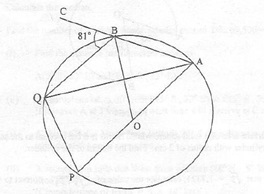
\includegraphics[width=5cm]{./img/circ1.jpg}
	\end{center}	
	
	\item The chords AB and CD of the circle given below meet at point O inside the circle. Given that AO = 8 cm, OC = 9 cm and OD = 4 cm, find OB.
	\begin{center}
	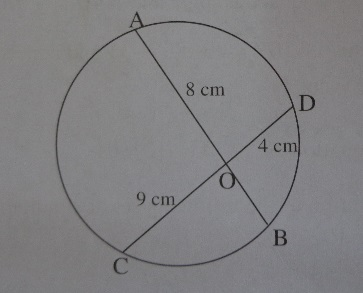
\includegraphics[width=5cm]{./img/circ19.jpg}
	\end{center}		

	\item In the figure below, O is the centre of the circle. Find the value of $x$.
	\begin{center}
	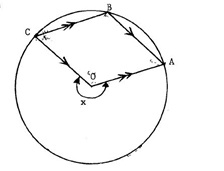
\includegraphics[width=5cm]{./img/circ2.jpg}
	\end{center}

	\item In the figure below ACD is an equilateral triangle and ABCD is a cyclic quadrilateral. Given that $E\hat{C}D = 20^\circ$, find the size of angle $E\hat{B}C$.
	\begin{center}
	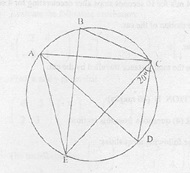
\includegraphics[width=5cm]{./img/circ3.jpg}
	\end{center}

	\item In the circle ABCD below, AB is an arc of $43^\circ$ and CD is an arc of $25^\circ$. O is the centre of the circle. What is the degree measure of $D\hat{L}C$?
	\begin{center}
	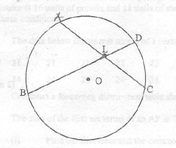
\includegraphics[width=5cm]{./img/circ4.jpg}
	\end{center}

	\item In the figure drawn here under, $\overline{AB} = 156$ mm, $\overline{CD} = 96$ mm and $\overline{PA}$ is 12 mm shorter than $\overline{PD}$. Find the length of $\overline{PA}$.
	\begin{center}
	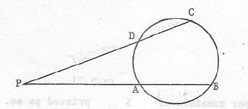
\includegraphics[width=5cm]{./img/circ5.jpg}
	\end{center}

	\item In the figure below, O is the centre of the circle, $A\hat{O}B = 120^\circ$ and $C\hat{D}B = 15^\circ$. Find the value of $x$.
	\begin{center}
	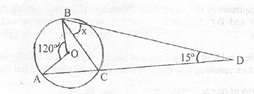
\includegraphics[width=6cm]{./img/circ6.jpg}
	\end{center}

	\item Determine the value of $x$ in the figure below where O is the centre of the circle.
	\begin{center}
	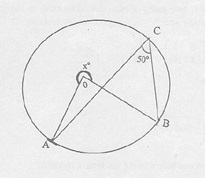
\includegraphics[width=5cm]{./img/circ7.jpg}
	\end{center}

	\item If, in the diagram below, ABCD is a cyclic quadrilateral, O is the centre and m$(A\hat{D}C) = 140^\circ$, find:\\
	(a) m$(A\hat{B}C)$ \quad (b) m$(A\hat{O}C)$ \quad (c) m$(O\hat{A}C)$
	\begin{center}
	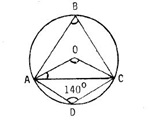
\includegraphics[width=5cm]{./img/circ8.jpg}
	\end{center}

	\item In the diagram below, $\overline{DC}$ is a diameter of the circle with centre O. The chord $\overline{AB}$ is parallel to $\overline{DC}$. Find the value of $x$ given that m$(A\hat{O}D) = 70^\circ$.
	\begin{center}
	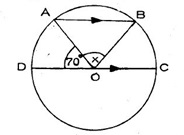
\includegraphics[width=5cm]{./img/circ9.jpg}
	\end{center}

	\item In the figure below find $x$.
	\begin{center}
	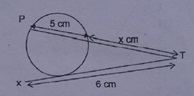
\includegraphics[width=5cm]{./img/circ10.jpg}
	\end{center}

	\item In the figure shown below, O is the centre of the circle, $A\hat{O}D = 100^\circ$ and $C\hat{D}B = 40^\circ$. Find the value of $x$ if AC is a line segment.
	\begin{center}
	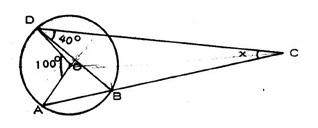
\includegraphics[width=6cm]{./img/circ11.jpg}
	\end{center}

	\item In the figure below, $\overline{AT}$ is the diameter of the circle. Points $A$, $B$ and $P$ lie on a straight line. $\overline{PT}$ is a tangent to the circle at $T$. If $AP = x$, $BP = b$ and $AT = y$, show that $y^2 = x^2 - bx$.
	\begin{center}
	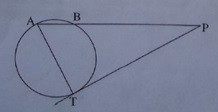
\includegraphics[width=5cm]{./img/circ12.jpg}
	\end{center}

	\item In the figure below, AC is the diameter of the circle ABCD and m$(D\hat{B}C) = 25^\circ$. Find m$(A\hat{C}D)$.
	\begin{center}
	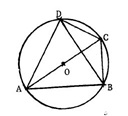
\includegraphics[width=4cm]{./img/circ13.jpg}
	\end{center}

	\item PQRS is a cyclic quadrilateral and PQ is produced to T. Prove that $R\hat{Q}T = P\hat{S}R$.
	\begin{center}
	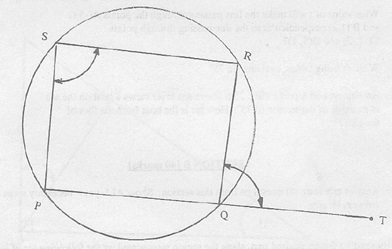
\includegraphics[width=5cm]{./img/circ14.jpg}
	\end{center}

	\item If ABCD is a circle with centre O and angle $C\hat{O}D = 130^\circ$, BD is a diameter and angle $B\hat{A}C = x^\circ$, calculate the value of $x^\circ$.
	\begin{center}
	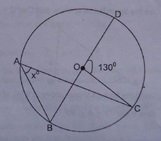
\includegraphics[width=4cm]{./img/circ15.jpg}
	\end{center}
	
	\item The two tangents AC and BC to the circle drawn below meet at C.
	\begin{center}
	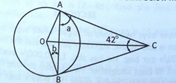
\includegraphics[width=5cm]{./img/circ16.jpg}
	\end{center}
	If O is the centre of the circle, calculate the size of the angles marked $a$ and $b$.
	
	\item Prove that the angles in the same segment of a circle are equal.
	
	\item Prove that the opposite angles of any quadrilateral inscribed in a circle are supplementary.
	
	\item Prove that the two tangents from an external point to a circle are equal.
	
	\item The end of a 60 cm pendulum describes an arc 5 cm long. Find the angle, in degrees, through which the pendulum swings.
	
	\item 
		\begin{itemize}
		\item[(i)] Change $315^\circ$ into radians (leave $\pi$ as $\pi$).
		\item[(ii)] Show that the radius of a circle with an arc of length $\pi$ m and central angle $\cfrac{\pi}{6}$ is 6 m.
		\end{itemize}
		
	\item The figure below shows that AO = OB = 7 cm, $A\hat{O}B = 36^\circ$ and O is the centre of the circle. Calculate the perimeter of the figure.
	\begin{center}
	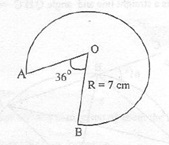
\includegraphics[width=3cm]{./img/circ17.jpg}
	\end{center}
	
	\item 
		\begin{itemize}
		\item[(a)] Below is a circle with centre O and radius $r$ units. By considering the circumference of the circle, the area of the circle, the given angle $\theta$ and the degree measure of the circle ($360^\circ$), develop the formula for finding:
		\begin{itemize}
		\item[(i)] Arc length AB
		\item[(ii)] Area of sector AOB.
		\end{itemize}
	\begin{center}
	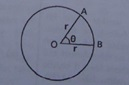
\includegraphics[width=3cm]{./img/circ18.jpg}
	\end{center}
	
		\item[(b)] Find:
			\begin{itemize}
			\item[(i)] The length of arc AB
			\item[(ii)] The area of the sector AOB
			\end{itemize}			 
			If $\theta$ is $57^\circ$ and $r$ is 5.4 cm $\left(\text{use } \pi = \cfrac{22}{7}\right)$.
			\end{itemize}
			
	\item Change each of the following angles which are in radians into degrees.
		\begin{itemize}
		\item[(i)] $\cfrac{7\pi}{4}$
		\item[(ii)] $\cfrac{5\pi}{9}$
		\end{itemize}
		
	\item Find the perimeter of a sector of a circle of radius 3.5 cm if the angle of the sector is $144^\circ$.

\end{enumerate}	
	
	
	
	\subsection{Earth as a Sphere}
\begin{enumerate}
	\item Find the distance (in km) between towns $P(12.4^\circ$S, $30.5^\circ$E$)$ and $Q(12.4^\circ$S, $39.8^\circ$E$)$ along a line of latitude, correctly to 4 decimal places.

	\item The location of Morogoro is $7^\circ$S, $38^\circ$E and that of Dar es Salaam is $7^\circ$S, $39^\circ$E. Find the distance between the two towns in kilometres.
	
	\item 
		\begin{itemize}
		\item[(i)] Find the distance in kilometres between A($9^\circ$S, $33^\circ$E) and B($5^\circ$S, $33^\circ$E).
		\item[(ii)] An aeroplane takes off from B($5^\circ$S, $33^\circ$E) to C($5^\circ$S, $39^\circ$E) at a speed of 332 km\slash h. If it leaves B at 3:00 pm, at what time will it arrive at C airport?
		\end{itemize}

	\item 
		\begin{itemize}
		\item[(i)] A ship sails due North from latitude $20^\circ$S for a distance of 1440 km. Find the latitude of the point it reaches.
		\item[(ii)] A second ship sails due West from position ($60^\circ$N, $5^\circ$W) for a distance of 1200 km. Find its new position.
		\end{itemize}
		(Circumference of Earth $= 4 \times 10^4$ km).
		
	\item A and B are two towns on latitude $42^\circ$N. If A is on the meridian $23^\circ$E and B is on $53^\circ$E,
		\begin{itemize}
		\item[(i)] Find the angle subtended by an arc AB
		\item[(ii)] Find the length of the arc AB in km.
		\end{itemize}
		
	\item Find the distance in km between Mbeya ($9^\circ$S, $33^\circ$E) and Tabora ($5^\circ$S, $33^\circ$E).
	
	\item Calculate the surface distance along latitude $30^\circ$N covered between longitudes $60^\circ$E and $65^\circ$W.
	
	\item Find the distance between A($30^\circ$N, $39^\circ$E) and B($45^\circ$S, $39^\circ$E) in
		\begin{itemize}
		\item[(i)] Nautical miles
		\item[(ii)] Kilometres
		\end{itemize}
		
	\item Calculate the volume of the earth.
	
	\item An aeroplane takes off from Tabora ($5^\circ$S, $33^\circ$E) to Tanga ($5^\circ$S, $39^\circ$E) at a speed of 332 km\slash h. If it leaves Tabora at 3:00 pm, at what time will it arrive at Tanga airport?
	
	\item 
		\begin{itemize}
		\item[(a)] A speed boat traveling from Zanzibar ($6^\circ$S, $45^\circ$E) to Mtwara ($9^\circ$S, $45^\circ$E) using 30 knots left Zanzibar at 11:30 am. At what time did it reach Mtwara?
		\item[(b)] Calculate the length of diameter (in kilometres) of the parallel of latitude $64^\circ$N.
		\item[(c)] Define the following terms:
			\begin{itemize}
			\item[(i)] Nautical mile
			\item[(ii)] Knot
			\end{itemize}
		\end{itemize}
		
	\item Given that the radius of the earth is 6400 km, find:
		\begin{itemize}
		\item[(i)] the length of the parallel latitude $30^\circ$N
		\item[(ii)] the shortest distance along the surface of the earth from town Q whose position is ($30^\circ$N, $10^\circ$E) to town P whose position is ($30^\circ$N, $50^\circ$W).
		\end{itemize}

	\item A and B are two points on latitude $70^\circ$N. Their longitudes are $62^\circ$W and $118^\circ$E respectively. Calculate the distance in kilometres from A to B if the Earth's diameter is 12800 km for the following cases:
		\begin{itemize}
		\item[(i)] Along a great circle route over the north pole.
		\item[(ii)] Along a parallel of latitude.
		\end{itemize}
		
	\item two place P and Q, both on the parallel of latitude $26^\circ$N differ in latitude by $40^\circ$. Find the distance between them along their parallel of latitude.

\end{enumerate}
	
	
	
	\subsection{Accounts}

\begin{enumerate}

	\item After Joachim completed form four in October 2010, he started chips business and he recorded the following transactions:\\
\begin{tabular}{l l l}
November & 1 &Started with capital of 260,000/=\\
& 2 & Purchased potatoes for cash 70,000/=\\
& 3 & Sold chips for cash 90,000/=\\
& 7 & Purchased cooking oil for cash 30,000/=\\
& 13 & Bought aluminum foil for cash 5,000/=\\
& 19 & Paid transport charge for cash 3,500/=\\
& 20 & Bought more potatoes for cash 20,000/=\\
& 24 & Paid rent for cash 6,000/=\\
& 27 & Sold chips for cash 60,000/=\\
\end{tabular}

	\begin{itemize}
	\item[(a)] Enter the above transactions in a Cash Account and show the business at 1\textsuperscript{st} December.
	\item[(b)] Open a Capital Account for the above business.
	\end{itemize}
	
	
	
	\item 
		\begin{itemize}
		\item[(a)] The following balances were extracted from the ledgers of Mr \& Mrs Mkomo business on 31\textsuperscript{st} January. Prepare the trial balance.\\
		\begin{tabular}{l r l r}
		Capital&30,000/=&Insurance&3,000/=	\\
		Furniture&25,000/=&Cash&18,000/=	\\
		Motor vehicle&45,000/=&Discount received&7,000/=	\\
		Sales&68,000/=&Discount allowed&4,000/=	\\
		Purchases&54,000/=&Drawing&12,000/=	\\
		Creditors&76,000/=&Electricity&5,000/=	\\
		Debtors&15,000/=&&	\\
		\end{tabular}
		\item[(b)] Determine the gross profit and the net profit from the information given below.\\
		\begin{tabular}{l r}
		Sales&38,000/= \\
		Opening stock&8,000/= \\
		Purchases&25,000/= \\
		Electricity&4,000/= \\
		Discount allowed&2,000/= \\
		Closing stock&5,000/= \\
		\end{tabular}
		\end{itemize}


	\item On 1st September 2006, the assets and liabilities of ABC Company were as follows:\\

\begin{tabular}{l r}
Cash in hand & 500 000\\
Cash at bank & 1 400 000\\
Debtor: T & 440 000\\
Debtor: Z & 400 000\\
Creditor: X & 670 000\\
Creditor: Y & 650 000\\
Stock & 450 000\\
Equipment & 700 000\\
Fixture and Fitting & 1 000 000\\
Motor Vehicle & 3 200 000\\
Premises & 5 200 000\\
\end{tabular}\\

Prepare the Balance Sheet of ABC Company as at 30 September 2006.


\item Study the given trial balance and answer the questions that follow.

\begin{center}
\begin{tabular}{|c|l|r|r|}
\multicolumn{4}{c}{\textbf{Trial Balance as at 31 December 2007}} \\\cline{1-4}
\textbf{S/N} &\multicolumn{1}{c|}{\textbf{Account Name}}&\multicolumn{1}{c|}{\textbf{Debit (Dr)}} & \multicolumn{1}{c|}{\textbf{Credit (Cr)}}\\ \cline{1-4}
1 & Cash  & 185 000 &  \\
2 & Capital &  & 200 000 \\
3 & Purchases & 110 000 &  \\
4 & Sales &  & 104 000 \\
5 & Water Bills & 3 000 &  \\
6 & Advertising & 2 000 &  \\
7 & Telephone Bills & 1 000 &  \\
8 & Salaries & 3 000 &  \\
\cline{1-4}
& & \textbf{304 000} & \textbf{304 000}\\ \cline{1-4}
\end{tabular}
\label{tab:prob2_tb}
\end{center}

Prepare the following for the year ending 31 December 2007:
\begin{itemize}
\item[(a)] Trading Account
\item[(b)] Profit and Loss Account
\item[(c)] Balance Sheet
\end{itemize}



\item From 1st January to 29th January 2006 Mr. Bin decided to keep record of his business as follows:\\

\begin{tabular}{c c l r}
Jan & 1 & Mr. Bin started business with capital in cash & 500 000/=\\
& 5 & Purchased goods & 254 000/=\\
& 6 & Sold goods & 290 000/=\\
& 9 & Purchased goods & 204 000/=\\
& 10 & Expenses & 24 000/=\\
& 29 & Sold goods & 320 000/=\\
\end{tabular}\\
\label{prob3_trans}

You are required to:
\begin{itemize}
\item[(a)] Prepare the Trial Balance
\item[(b)] Open the Capital and Cash Account
\end{itemize}
\textit{\textbf{N.B.} All payment and receipt were made in cash.}


\item The following information relates to Mr. Kazimoto, a trader, as at 30th July 2004:\\

\begin{tabular}{l p{4cm} m{1cm} l}
Sales: & shs. 340 000 && \textit{Calculate:}\\
Cost of sales: & 75\% of sales && (a) Purchases\\
Opening Stock: & shs. 90 000 && (b) Cost of sales\\
Net Profit: & 20\% of sales & &(c) Closing Stock\\
Closing Stock: & 20\% of cost of goods sold && (d) Net Profit\\
 &  & &(e) Expenses\\
\end{tabular}



\item At the bearing of August 2008, Nguvumpya Secondary School started up a school project shop with a capital of Tshs. 1,800,000/=. The school project manager made the following transactions.\\

\begin{tabular}{l p{13cm}}
On August 6th & she bought some stationeries for the shop worth Tshs. 180,000/=\\
On August 9th & she sold goods to the students worth Tshs. 270,000/=\\
On August 11th & she bought soft drinks for the shop from the IPP Company worth Tshs. 630,000/=\\
On August 13th & she sold foodstuffs to teachers worth Tshs. 450,000/=\\
On August 15th & she sold foodstuffs to villagers worth Tshs. 360,000/=\\
On August 17th & she bought loaves of bread for the shop worth Tshs. 450,000/=\\
On August 19th & paid transport charges Tshs. 50,000/= and the shop management paid wages to the shop manager Tshs. 90,000/= on August 28th.
\end{tabular}

\begin{itemize}
\item[(a)] Enter these transactions in a cash book.
\item[(b)] Bring down the balance at the end of August 28th 2008.
\end{itemize}




\item Enter the following items in a cash a\slash c balance, off at the end, and bring the balance.\\

\begin{tabular}{l l p{4cm} r}
Jan 1996:&  & & \\
& January 1st & balance of cash in hand & 6,000/=\\
& January 2nd & we paid for repairs & 250/=\\
& January 3rd & we paid garage expenses & 750/=\\
& January 4th & cash sales & 2,500/=\\
& January 5th & we paid wages & 300/=\\
& January 6th & we paid Anna & 150/=\\
& January 7th & we paid John & 1,300/=\\
& January 8th & we paid office expenses & 175/=\\
& January 9th & cash sales & 1,500/=\\
& January 10th & Samwel paid us & 1,400/=\\
& January 11th & we received from Asha & 1,500/=\\
& January 12th & we paid Peter & 2,500/=\\
& January 13th & we paid for office expenses & 75/=\\
& January 14th & cash sales & 2,300/=
\end{tabular}



\item Record the following transactions per the month of February 2010.\\

\begin{tabular}{lll}
February: & &\\
& 1 & Started business with 50,000/= in the bank\\
& 2 & Bought motor van paying by cheque 12,000/=\\
& 6 & Took 20,000/= out of the bank and put it into the cash\\
& 10 & Bought office equipment paying by cash 6,000/=\\
& 18 & Cash sales 8,000/=\\
& 19 & Paid motor expenses for cash 4,700/=\\
& 27 & Paid rent for cash 540/=\\
& 28 & Komba paid us a cheques of 9,800/=\\
\end{tabular}


\end{enumerate}

\section{Form IV}

	\subsection{Coordinate Geometry} \label{f4coordgeo}
	
\begin{enumerate}
	
%slope-intercept form	
		\subsubsection{Slope / Equation of a Line}
	\item Find the y-intercept and the gradient of the line which passes through the points (7,5) and (2,3).
	
	\item A line whose equation is $y = mx + c$ passes through (-1,4). If x-intercept for this line is 3, determine the values of $m$ and $c$.
	
	\item The straight line through the points C(1,-2) and D(3,4) meets the y-axis at point E. Find the coordinates of E.
	
	\item Determine the slope of the line $\frac{7}{2}x - \frac{5}{3}y - 4 = 0$.
	
	%line segments	
	\item The coordinates of the points O, P, Q and R are (0,0), (2,-1), (3,2) and (13,4) respectively and $\overline{OR} = a \overline{OP} + b \overline{OQ}$. Find the value of each of the scalars $a$ and $b$.
	
	%triangles / angles
	
	
	\item Write down the equation of the line which passes through (7,3) and which is inclined at 45$^\circ$ to the positive direction of the x-axis.
	
	\item Find an equation of a line passing through point (3,4) and its inclination is 45$^\circ$.
	
	
%midpoint	
		\subsubsection{Midpoint}
	\item Find the coordinates of the midpoint of the line joining the points (-2,8) and (-4,-2).
	
	\item Find the equation of the straight line joining the point O(0,0) to the mid-point of the line joining A(3,2) and B(5,-1).
	
	\item The line defined by the equation $x + y = 12$ crosses the y-axis at A and meets the line $x = 6$ at B. If C is the point (0,3) and M is the midpoint of $\overline{AB}$, find:
	\begin{itemize}
	\item[(a)] the coordinates of A, B and M
	\item[(b)] the equation of the line $\overline{CM}$
	\item[(c)] the equation of the line which is perpendicular to the line $\overline{CM}$ passing through M.
	\end{itemize}
	
	
%distance	
		\subsubsection{Distance Between Two Points}
	\item Find the distance between the point (-3,-2) and the point midway between (2,13) and (4,7). Write your answer in the form $a\sqrt{c}$ wher $a$ and $c$ are positive real numbers.
	
	\item Find the distance between the points A(3,7) and B(-2,-5).
	
	\item The coordinates of the points A, B and C are (4,3), (3,-2) and (7,-1) respectively. From this information find the:
	\begin{itemize}
	\item[(a)] length of AB
	\item[(b)] equation of the line BC. (Write your answer in the form $ax + by + c = 0$).
	\end{itemize}
	
	\item Find the coordinates of a point of a line presented by $2x - 3y + 7 = 0$, which is equi-distant from the points (-4,-8) and (7,1).
	
%parallel, perpendicular	
		\subsubsection{Parallel / Perpendicular Lines}
	\item Find the equation of a straight line that is parallel to the line $3x + 4y = 1$ and cuts the x-axis where $x = -1$. Express your answer in the form $ax + by + c = 0$ where $a$, $b$ and $c$ are constants.
	
	\item Determine the equation of a line which passes through the point N(5,0) and is parallel to the line $3x + 4y = 12$.
	
	\item The line passing through the points A(k,4) and B(3,2k) is parallel to the line $y + 3x - 4 = 0$. Find the value of k.
	
	
	

	\item The gradient of line $l_1$ is -2. Another line, $l_2$, is perpendicular to $l_1$ and passes through (-3,-2). What is the equation of $l_2$?
	
	\item 
	\begin{itemize}
	\item[(a)] What value of K will make the line containing the points (K,5) and (-2,3) parallel to the line containing the points (6,K) and (2,0)?
	\item[(b)] What value of K will make the lines perpendicular to each other?
	\end{itemize}
	
	\item The line $l$ is perpendicular to the line $y = 4x - 5$. If $l$ passes through the point (-4,4), find its equation.
	
	\item Find the equation of the line passing through the point (-3,8) which is perpendicular to the line defined by the equation $y = 3x - 4$.
	
	\item Both lines ``r'' and ``s'' pass through the point (k,9). Line ``r'' has a slope of $-\frac{4}{3}$ and passes through the point (5,-3). Determine the:
	\begin{itemize}
	\item[(a)] value of k.
	\item[(b)] equation of ``s'' in standard form of $ax + by + c = 0$, if its x-intercept is -14.
	\item[(c)] equation of line ``t'' perpendicular to line ``r'' which passes through the point (k,9) if form of $y = mx + c$.
	\end{itemize}
	
	\item Find the equation of the perpendicular bisector of the line joining a line segment whose end-points have coordinates (0,2) and (3,6). Put it in the form $y = ax + b$.
	
	\item Find the equation of the perpendicular bisector of the line joining the points A(3,-1) and B(-5,2), in the form $y = mx + c$ where $m$ and $c$ are constants.
	
	\item Find the equation of a line through the point (2,3) perpendicular to the line whose equation is $4y - 3x + 1 = 0$.
	
	\item What value of t will make the line passing through the points A(-5,t) and B(1,2) perpendicular to the line passing through points C(-1,-2) and D(5,1)?
	
	\item A straight line through (13,2) intersects perpendicularly the line $3x - 2y + 4 = 0$. Find the equation of this perpendicular line and write the equation in standard form.
	
	\item Line L is perpendicular to the line joining the points (-3,2) and (5,6). If it passes through the point of intersection of the lines $2x - y = 1$ and $3x + 3y - 6 = 0$, determine the equations of line L.
	
	\item 
	\begin{itemize}
	\item[(a)] $L_1$ and $L_2$ are two lines which intersect each other at a right angle at the point (1,3). $L_1$ cuts the y-axis at the point (0,2). Find the equation of $L_1$ and $L_2$.
	\item[(b)] By plotting the equations $L_1$ and $L_2$ on the same axes, demonstrate that the solution of simultaneous equations can be obtained graphically.
	\end{itemize}
	
	\item Determine the coordinates of the point P($x$,$y$) on the y-axis such that the line joining it to the point (3,-1) forms a right angle with the line through the points (3,-1) and (-5,-5).	
	
	\item The point A(5,-7) is the vertex of the right angle of a right angles triangle whose hypotenuse lies along the line $6x - 13y = 39$. A second vertex of the triangle is B(0,-3). Find the remaining vertex C($x$,$y$).	
	




\end{enumerate}	
	
	\subsection{Area and Perimeter} \label{f4ap}
\begin{enumerate}

	\item Calculate the perimeter of a regular polygon whose angle is $160^\circ$ and whose side is 5 cm.
	
	\item The diagonals of a rhombus are 16 cm and 12 cm long. Find the area and perimeter of the rhombus.
	
	\item Find the area and the perimeter of the parallelogram ABCD given in the figure below if $B\hat{A}D = 45^\circ$.
	\begin{center}
	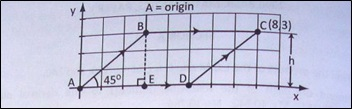
\includegraphics[width=7cm]{./img/ap1.jpg}
	\end{center}

	\item In the figure below, the area of the shaded part DEA is 15 m$^2$. If DA = 3 m and AB = 6 m, find the area of the quadrilateral BCDE.
	\begin{center}
	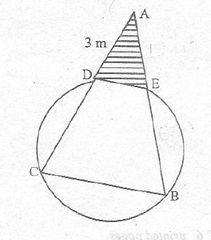
\includegraphics[width=4cm]{./img/ap2.jpg}
	\end{center}

	\item A regular pentagon is inscribed in a circle of radius 10 cm.
		\begin{itemize}
		\item[(a)] Draw a diagram to show the regular pentagon inscribed in the circle.
		\item[(b)] Calculate the area of the region outside the regular pentagon but inside the circle. (use $\pi = 3.14$)
		\end{itemize}
		
	\item The height of a trapezium is 13 cm. If one of its parallel sides is 20 cm and the area of the trapezium is 390 cm$^2$, find the length of the other parallel side.
	
	\item Find the area of $\bigtriangleup ABC$ given that $AB = 4$ cm, $BC = 7$ cm and m$(A\hat{B}C) = 30^\circ$.
	
	\item In the diagram drawn below, ABCD is a parallelogram in which AD is extended to E. The area of the parallelogram is 40 cm$^2$. Determine the area of $\bigtriangleup$ DCE given that AE = 11 cm and BC = 8 cm.
	\begin{center}
	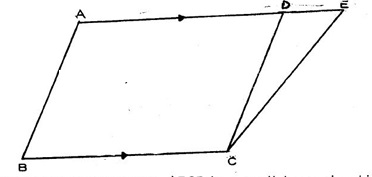
\includegraphics[width=5cm]{./img/ap3.jpg}
	\end{center}
	
	\item Find the area of triangle $ABC$ if $\overline{AB} = 4$ cm, $\overline{BC} = 7$ cm and m$(A\hat{B}C) = 30^\circ$.
	
	\item What is the area of a regular 45 sided polygon inscribed in a circle of radius 6 cm?

	\item What is the area of a regular 36 sided polygon inscribed in a circle of radius 10 cm?
	
	\item A regular hexagonal piece of paper has a circular hole of radius 2 cm at the centre. Each side of the regular hexagon is 6 cm long. Find the area of this piece of paper in cm$^2$ correct to 1 decimal place.
	\begin{center}
	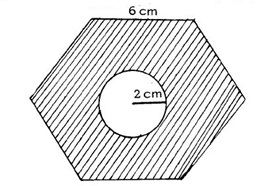
\includegraphics[width=5cm]{./img/ap4.jpg}
	\end{center}

	\item A circle of radius 10 units is circumscribed by a right-angled isosceles triangle. Find the lengths of the sides of the triangle and hence its perimeter (all in 2 decimal places).

\end{enumerate}	
	
	
	
	\subsection{Three-Dimensional Figures}
\begin{enumerate}

	\item An open rectangular box measures externally 32 cm long, 27 cm wide and 15 cm deep. If the box is made of wood 1 cm thick, find the volume of wood used.

	\item For a tank given in the figure below, calculate the angle between $\overline{DF}$ and the base ABCD.
	\begin{center}
	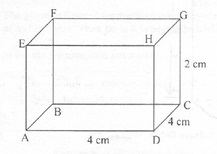
\includegraphics[width=5cm]{./img/3d1.jpg}
	\end{center}

	\item The volume of a rectangular box is 1008 cm$^3$. If its length is 14 cm and its breadth is 9 cm, find its height.
	
	\item A rectangular box with top WXYZ and base ABCD has AB = 6 cm, BC = 8 cm and WA = 3 cm.
	\begin{center}
	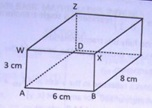
\includegraphics[width=5cm]{./img/3d2.jpg}
	\end{center}

	Calculate:
	\begin{itemize}
	\item[(i)] Length of AC
	\item[(ii)] Angle between WC and AC
	\end{itemize}
	
	\item The figure below shows a rectangular prism in which $\overline{AB} = 16$ cm, $\overline{BC} = 12$ cm and $\overline{QC} = 5$ cm.
	\begin{center}
	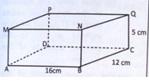
\includegraphics[width=5cm]{./img/3d3.jpg}
	\end{center}

	Calculate:
	\begin{itemize}
	\item[(a)] its total surface area
	\item[(b)] the angle between $\overline{PB}$ and the base ABCD
	\item[(c)] the volume in litres the prism can hold (1 litre = 1000 cm$^3$)
	\end{itemize}
	
	\item In the figure below ABCD is a rectangle in which AB = 3 cm and BC = 2 cm. V is a point such that VA = VB = VC = VD = 6 cm and AO = OC. Find:
		\begin{itemize}
		\item[(a)] The angle VAD
		\item[(b)] The length of AC
		\item[(c)] The angle between VA and the plane ABCD
		\end{itemize}
	\begin{center}
	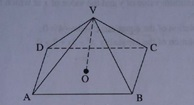
\includegraphics[width=5cm]{./img/3d4.jpg}
	\end{center}

	\item In the diagram below, VABCD is a pyramid whose base ABCD is a square with sides 6 cm. The vertex V is vertically above N, the centre of the base and VN = 3 cm.
	\begin{center}
	\includegraphics[width=5cm]{./img/3d5.jpg}
	\end{center}
	Calculate:
	\begin{itemize}
	\item[(a)] length VA
	\item[(b)] angle between the line VA and the plane ABCD
	\item[(c)] volume of the pyramid.
	\end{itemize}
	
	\item A pyramid has a square base ABCD of side 10 cm. The vertex V is 12 cm above the centre of the base E.
		\begin{itemize}
		\item[(i)] Find the angle of inclination of VA to the horizontal.
		\item[(ii)] Calculate the volume of the pyramid.
		\end{itemize}
		
	\item ABCDV is a right square pyramid where ABCD is the square base with BC and AD being diagonals and V the vertex which is 6 cm vertically above the centre E of the base.
		\begin{itemize}
		\item[(a)] Draw a three dimensional diagram of the pyramid.
		\item[(b)] Calculate:
			\begin{itemize}
			\item[(i)] the length BV
			\item[(ii)] the angle between the planes AVC and BVD
			\item[(iii)] the volume of the pyramid.
			\end{itemize}
		\end{itemize}
		
	\item The diagram below represents a right pyramid with a rectangular base PQRS and vertex V. Each slanting edge is 12 cm long. PQ = 8 cm and QR = 6 cm. Calculate:
		\begin{itemize}
		\item[(a)] the angle between VPQ and the base PQRS.
		\item[(b)] the total surface area of the pyramid.
		\end{itemize}
	\begin{center}
	\includegraphics[width=6cm]{./img/3d6.jpg}
	\end{center}

	\item The surface area of a solid sphere whose radius is 6 cm is equal to the surface area of a solid right cylinder with radius of 2 cm. Find the height of the cylinder.
	
	\item 
		\begin{itemize}
		\item[(a)] The total surface area of a solid cylinder is 748 cm$^2$. The surface area of the circular faces is 308 cm$^2$. Find the height of the cylinder.
		\item[(b)] Given that the surface area of a sphere is given by $S = 4\pi r^2$ and volume by $V = \cfrac{4}{3}\pi r^3$, show that $V = \cfrac{1}{6}\left(\cfrac{\sqrt{s^3}}{\pi}\right)$.
		\end{itemize}
		
	\item Find the volume of the metal needed to make 1000 ball bearings of diameter 4 mm.
	
	\item A sphere of diameter 4 cm is beaten out into a circular sheet 0.03 cm thick. Find the radius of the sheet.
	
	\item Calculate the volume and surface area of a sphere of radius 210 cm.
	
	\item A sphere is cut by a horizontal plane so that the area of the cross section is 81$\pi$ cm$^2$. If the distance from the plane to the centre is 15 cm, find the radius of the sphere.
	
	\item The volume of two similar cylinders is 125 cm$^3$ and 512 cm$^3$. If the radius of the larger cylinder is 8 cm, find the radius of the smaller cylinder.
	
	\item A cylinder of base radius of 14 cm has a height of 28 cm. Calculate its volume.
	
	\item The curved surface area of a cylinder is 264 cm$^2$. If the height of the cylinder is 14 cm, calculate its volume and radius.
	
	\item A cylindrical solid of radius 7 cm and height 25 cm is cut equally from the top to bottom resulting into equal half solids (see figure below). Find the total surface area of one half solid. $\pi = \cfrac{22}{7}$ may be used.
	\begin{center}
	\includegraphics[width=4cm]{./img/3d7.jpg}
	\end{center}

	\item Find the capacity in litres of a bucket 24 cm in diameter at the top, 16 cm in diameter at the bottom and 18 cm deep.
	
	\item A piece of metal 12 cm long, 8 cm wide and 3 cm thick is melted and recasted into a cone whose base area is 36 cm$^2$. Find the height of this cone.
	
	\item The total surface area of a solid cone is 440 cm$^2$. The length of the diameter of its circular region is 14 cm. Calculate the length of the slant edge.
	
	\item Find the total surface area of a right circular cone whose height is 24 cm and slant height is 25 cm.
	
	\item Find the area of the curved surface of a cone whose base radius is 3 cm and whose height is 4 cm.

\end{enumerate}	
	
	
	
	
	\subsection{Probability}
\begin{enumerate}
%single simple events

	\item A bag contains 4 red, 2 white and 2 blue balls. A ball is drawn at random from the bag. Find the probability that it is not blue.
	
	\item A box has 8 red balls and 11 white balls of the same size. A ball is drawn at random from the box. What is the probability that it is
	\begin{itemize}
	\item[(i)] red
	\item[(ii)] white?
	\end{itemize}
	
	\item A fair die is tossed once and the number showing up is recorded. What is the probability of an even number greater than two showing up?
	
	\item The four congruent faces of a tetrahedron are marked 1, 2, 3 and 4 respectively. What is the probability that when the tetrahedron is tossed it will show a prime number?
	
	\item An integer is selected at random from the numbers lying between 50 and 60 inclusive. Find the probability that the selected number is:
		\begin{itemize}
		\item[(i)] prime
		\item[(ii)] a multiple of four
		\item[(iii)] a multiple of five
		\item[(iv)] a square of a whole number.
		\end{itemize}
		
		\item Find the probability that a number chosen at random from a set of integers between 10 and 20 inclusive is either a prime number or a multiple of five.
		
		\item The numbers 1 to 20 are each written on a card. The 20 cards are then mixed together. One card is chosen at random from the pack. Find the probability that the number on the card is:
	\begin{itemize}
	\item[(i)] Even
	\item[(ii)] A factor of 24
	\item[(iii)] Prime
	\end{itemize}
	
	\item If $D = \{x: 80\leq x \leq 100\}$, find the probability that the number selected from D is:
	\begin{itemize}
	\item[(i)] divisible by 7
	\item[(ii)] a prime number
	\item[(iii)] an odd number.
	\end{itemize}
			
	\item Find the probability that a number selected at random from the numbers -3, -2, 0, 3, 4 and 6 will be a solution set of the equation $x^2 - x - 6 = 0$.
	
	
%multiple simple events	
	\item Two numbers are chosen at random from 1, 2 and 3. What is the probability that their sum is odd?
	
	\item A pair of dice is thrown. Find the probability that the sum is 10 or greater if a 5 appears on the first die.
	
	\item Two dice are rolled together. Find the probability of the following:
		\begin{itemize}
		\item[(a)] that both faces show even numbers
		\item[(b)] that one face shows an even number and the other one an odd number
		\item[(c)] that the sum of the scores on the two faces is 9.
		\end{itemize}
	
	\item A fair die and coin are tossed once. What is the probability of a head on the coin and an even number of the die showing up?
			
	\item A black die and a white die are thrown at the same time. Find the probability of obtaining a total of (i) 5 (ii) 11.
	
	\item A box contains 7 red balls and 14 black balls. Two balls are drawn at random without replacement.
		\begin{itemize}
		\item[(a)] Draw a tree diagram to show the results of the drawing.
		\item[(b)] Find the probability that both are black.
		\item[(c)] Find the probability that they are of the same colour.
		\item[(d)] Find the probability that the first is black and the second is red.
		\item[(e)] Verify the probability rule $P(A) + P(A') = 1$ by using the results in part (b).
		\end{itemize}
	
	\item A box contains 4 white balls and 5 black balls. Two balls are drawn at random from the box. Find the probability that both balls drawn are:
		\begin{itemize}
		\item[(i)] white
		\item[(ii)] black
		\end{itemize}
	
	\item 
	\begin{itemize}
	\item[(a)] A fraction is written by selecting the numerator from the digits 1, 2, 3 and the denominator from the digits 6, 8.\\
	\noindent Find the probability that the fraction written is less than $\frac{1}{2}$.
	\item[(b)] Box A contains 8 items of which 3 are defective and Box B contains 5 items of which 2 are defective. An item is drawn at random from each box. What is the probability that:
		\begin{itemize}
		\item[(i)] both items are non-defective?
		\item[(ii)] one item is defective and one item is not defective?
		\end{itemize}
	\end{itemize}	 
		
	\item A box has 8 red balls and 11 white balls of the same size. Two balls are drawn at random from the box one after another without replacement. What is the probability that:
		\begin{itemize}
		\item[(i)] All balls are red
		\item[(ii)] At least one white ball is drawn
		\end{itemize}
		
	\item A box contains 9 oranges, 7 mangoes and 2 lemons. A fruit is drawn at random and then replaced. Another draw is made. What is the probability that both fruits drawn are not mangoes?	
	
	\item 
	\begin{itemize}
	\item[(a)] A two digit number is written using the numbers 2, 3 and 4 without repetition.\\
	\noindent Find the probability that the number is:
		\begin{itemize}
		\item[(i)] even.
		\item[(ii)] less than 30.
		\end{itemize}
	\item[(b)] A family has four children. By using a tree diagram, find the probability that the family has:
		\begin{itemize}
		\item[(i)] all boys.
		\item[(ii)] two boys and two girls.
		\end{itemize}
	\end{itemize}
	
	
%defective, non-defective
	\item Three defective transistors and two good transistors are mixed in a box. Two transistors are randomly selected. Find the probability that they are both defective if the selections are made
	\begin{itemize}
	\item[(i)] with replacement
	\item[(ii)] without replacement
	\end{itemize}
	
	\item Box A has 10 light bulbs of which 4 are defective and box B has 6 light bulbs of which 1 is defective. If a box is selected at random and then a bulb is randomly drawn, calculate the probability that both drawn are defective.
	
	\item At a second-hand car show, 20\% of the cars have no engine, 40\% have bad tyres and 15\% have no engine and have bad tyres. What is the probability that a car chosen at random has good tyres and an engine?
	
	
%students in class	
	\item The table shows a distribution of students in each age group in a class.
	\begin{center}
	\begin{tabular}{|l|c|c|c|c|} \hline
	Age group & 16 & 17 & 18 & 19 \\ \hline
	Number of students & 7 & 22 & 13 & 0\\ \hline
	\end{tabular}
	\end{center}
	\noindent What is the probability that a student chosen from a class
	\begin{itemize}
	\item[(i)] is 17 years old?
	\item[(ii)] is over 16 years old?
	\end{itemize}
	
	\item The probability that Rose and Juma will be selected for A-level studies after completing O-level studies are 0.4 and 0.7 respectively. Calculate the probability that:
	\begin{itemize}
	\item[(i)] both of them will be selected
	\item[(ii)] either Rose or Juma will be selected
	\end{itemize}
	
	\item 
	\begin{itemize}
	\item[(a)] If the probability that Ali will pass Mathematics is 0.3 and the probability that he will pass Biology is 0.6, find the probability that:
		\begin{itemize}
		\item[(i)] He will pass both subjects
		\item[(ii)] He will fail both subjects
		\end{itemize}
	\item[(b)] If A is the event ``Ali will pass Mathematics'' and B is the event ``Ali will pass Biology'' show whether or not A and B are independent events (Use the information given in part (a) above).
	\end{itemize}
	
	\item Juma and Gadi are about to sit for CSEE. Juma says, ``I have a 50\% chance of passing my examinations.'' Gadi says, ``Probability of failing my examinations is $\frac{1}{4}$.'' Find the probability that:
		\begin{itemize}
		\item[(i)] Gadi will pass the examinations.
		\item[(ii)] Either Juma will pass the examinations or Gadi will fail the examinations.
		\end{itemize}

	\item The probability that Joti goes swimming on any day is 0.2. On a day when he goes swimming, the probability that he has chips for supper is 0.75. On a day when he does not go swimming the probability that he has chips for supper is x. This information is shown on the following tree diagram.
	\begin{center}
	\includegraphics[width=5cm]{./img/prob1.jpg}
	\end{center}
	
	\noindent The probability that Joti has chips for supper on any day is 0.5.
	\begin{itemize}
	\item[(i)] Find x.
	\item[(ii)] Suppose that Joti has chips for supper. Find the probability that he went swimming that day.
	\end{itemize}
	
	
	
	
	\item A box contains 40 identical discs, some of them being white and the rest blue. If a disc is drawn at random, the probability that it is white is $\frac{4}{5}$.
	\begin{itemize}
	\item[(a)] How many blue discs are there in the box?
	\item[(b)] How many blue discs should be added into the box to make the probability of drawing a blue disc $\frac{1}{3}$?
	\item[(c)] After removing 2 white and 3 blue discs from the box what will be the probability of drawing a white disc?
	\end{itemize}

	
	
	
	
	
	
	
% how many can be formed using digits
	
	\item 
	\begin{itemize}
	\item[(a)] How many different three-digit numerals can be formed by using the digits 3, 4, 6, 7 and 9 if no digit may be repeated in the same numeral?
	\item[(b)] How many numerals formed in part (a) are greater than 500?
	\item[(c)] Hence find the probability of forming a three-digit numeral greater than 500 using the digits 3, 4, 6, 7 and 9 without repeating a digit in the same numeral.
	\item[(d)] Answer part (c) if digits may be repeated.
	\end{itemize}
	
	\item
	\begin{itemize}
	\item[(a)] How many four digit numbers can be formed from the digits 2, 3, 4, 5 and 6 if the digits may not be repeated in the same numeral?
	\item[(b)] How many four digit numbers greater than 3000 can be formed from the digits 2, 3, 4, 5 and 6 if the digits may not be repeated in the same numeral?
	\item[(c)] Find the probability of forming a four digit number greater than 3000, if digits may not be repeated in the same numeral.
	\item[(d)] Repeat (c) above if the digits may be repeated in the same numeral.
	\end{itemize}
	
	\item A two-digit numeral is written using the digits \{2,3,4,5,6\}. What is the chance that a numeral written is less than 40 if a digit may not be repeated?
	
	\item How many even numbers greater than 2000 can be formed with the digits 1, 2, 4 and 8 if each digit may be used only once?
	
	\item How many arrangements are there of the letters of the word ``SOLOPAGA''?
	
	\item In a class of thirty pupils, one prize is awarded for English, another for Kiswahili, and a third for Mathematics. In how many ways can the winners be chosen?
	
	\item A girl has two jackets, four nice blouses, and three pairs of good shoes. How many different outfits, consisting of a jacket, blouse, and a pair of shoes, can she make out of these?
	
	\item A boy has five different flags. In how many ways can he fly them one above the other?


%sets, union	
	\item Given that $P(A') = \frac{1}{6}$, $P(B') = \frac{3}{5}$ and $P(A\cap B) = \frac{1}{4}$. Find $P(A\cup B)$.

	\item If A and B are two events such that $P(A) = \frac{1}{4}$, $P(B) = \frac{1}{2}$ and $P(A\cap B) = \frac{1}{8}$, find:
	\begin{itemize}
	\item[(i)] $P(A\cup B)$
	\item[(ii)] $P(A\cup B)'$
	\end{itemize}

\end{enumerate}


	\subsection{Trigonometry} \label{f4trig}
\begin{enumerate}

	\item Given that $\theta$ is an acute angle and $\sin \theta = \cfrac{3}{5}$, find the value of $\cfrac{\cos \theta - \sin \theta}{\tan \theta}$.

	\item Given that $\sin A = \cfrac{3}{5}$ find the values of:
		\begin{itemize}
		\item[(i)] $\cos A$
		\item[(ii)] $\cfrac{\tan A - \sin A}{1 + \cos A}$
		\end{itemize}

	\item If $5\cos A = 3$ find the values of:\\
	(i) $\sin A$ \quad	(ii) $\tan A$
	
	\item Let $A$ be the acute angle of a right angles triangle ABC such that $\hat{B} = 90^\circ$ and $\cos \hat{C} = \cfrac{5}{13}$. Find the value of $\sin \hat{A}$.
	
	\item Given that $x$ is an acute angle and that $\sin x = \cfrac{p}{q}$, find the value of $\tan x$.
	
	\item If $\tan A = 2\cfrac{2}{5}$ where $A$ is an acute angle, find:\\
	(i) $\sin A$ \quad and \quad (ii) $\cos A$
	
	\item If $N$ is an acute angle and $\tan N = \cfrac{5}{13}$, without using tables, find the value of $\sin N + 5\cos N$.
	
	\item Find the value of:
		\begin{itemize}
		\item[(i)] $\sin A$
		\item[(ii)] $\cos A$, if $\tan A = -\cfrac{5}{12}$ and it is known that $A$ is obtuse.
		\item[(iii)] Hence show that $13\sin A + 13\cos A = -7$.
		\end{itemize}

	\item If $\tan A = \cfrac{3}{4}$ and $A$ is acute, find $\cos A$, $\sin A$ and hence verify the identity $\cos^2 A + \sin^2 A = 1$.
	
	\item If $2\sin A = 1$ and $A$ is an obtuse angle, find the value of\\
	(a) $\cos A$ \quad (b) $\tan A$
	



%interval 0 - 360
	\item Show that $\sin(x + 10^\circ) = \cos(80^\circ - x)$ and hence find the value of $x$ for which $\sin(x + 10^\circ) = \cos 4x$.

	\item Find the values of $\theta$ between $0^\circ$ and $360^\circ$ which satisfy the equation:\\
	$\cos^2 \theta = 3(1 + \sin \theta)$.
	
	\item Given the value of $\tan \theta = -1$, find the possible values of $\theta$ in the interval $0^\circ \leq \theta \leq 360^\circ$.
	
	\item Find the truth set of $\sin \theta = -\cfrac{1}{2}$ in the domain $0^\circ \leq \theta \leq 360^\circ$.
	
		\item Without mathematical tables, find the numerical value of\\
	$\cfrac{1}{\sin^2 45^\circ} + \cfrac{2}{\cos^2 45^\circ} + \cfrac{3}{\tan^2 45^\circ}$
	
	\item Without using tables, simplify: $\cfrac{\sin 30^\circ \cos 30^\circ}{\tan 30^\circ}$.
	
	\item If $\tan^2 A + 2\tan^2 B + 3 = 0$, show that $\cos^2 B + 2\cos^2 A = 0$.
	
	\item Solve for $x$ if $2\sin^2 x - \cos x - 1 = 0$, for $0^\circ \leq x \leq 360^\circ$.
	
	\item Solve for $x$ if $\sin 3x = \cos 2x$ and $0^\circ \leq x \leq 90^\circ$.
	
	\item Without using tables, evaluate $\sin 75^\circ$.
	
	\item Factorise the expression: $\cos^4 x - \sin^4 x$.
	
	\item Simplify the expression: $\cfrac{\sin^4 x - \cos^4 x}{\sin^2 x - \cos^2 x}$
	
	\item Show that $(\cos \theta + \sin \theta)^2 + (\cos \theta - \sin \theta)^2 = 2$.
	
	\item Verify that for any angle $A^\circ$: $\cos (90^\circ - A^\circ) = \sin A^\circ$.
	
	\item Given that $\cos (90^\circ - \theta) = \cfrac{1}{2}\sqrt{3}$ where $\theta$ is an acute angle, without using tables, find the value of $\cos \theta$.
	
	\item Find without using tables, the value of $\tan \theta$, given that: \\
	$\tan (\theta - 45^\circ) = \cfrac{1}{3}$.
	
%word probs	
	\item A ladder reaches the top of a wall 18 m high when the other end on the ground is 8 m from the wall. Find the length of the ladder.

	\item Joff is 30 m from a flag pole installed with its bottom end some distance below ground level. The angle of elevation of the top of the flag pole from Joff's eye level is $12.4^\circ$ and the angle of depression of its bottom end is $2.1^\circ$. Calculate the height of the flag pole.
	
	\item The angle of elevation of the top of a tower from a point on the ground 80 m from the foot of the tower is $45^\circ$. Find the height of the tower.
	
	\item An observer on top of a cliff, 25 m above sea level, views a boat on the sea at an angle of depression of $75^\circ$. How far is the boat from the foot of the cliff?
	
	\item An observer on the top of a cliff, 25 m above sea level, views a boat on the sea at an angle of depression of $60^\circ$. How far is the boat from the top of the cliff?
	
	\item The figure below represents plotting of two stations A and B which are 4,000 m apart. T is a stationary target in the same vertical plane as A and B. When the distance of the target from station A is 10,000 m the angle of elevation is $30^\circ$. Calculate:
		\begin{itemize}
		\item[(a)] the vertical height of the target, TX
		\item[(b)] the distance AX, BX and TB
		\item[(c)] the angle of elevation of the target, T, from B
		\end{itemize}
	\begin{center}
	\includegraphics[width=5cm]{./img/trig3.jpg}
	\end{center}

	\item A man is standing 10 metres from a tree which is perpendicular to the ground. The angle of elevation of the top of the tree from the point on the ground where the man is standing is $21^\circ 48'$. What is the height of the tree?
	
	\item To find the height of a tower a surveyor sets up his theodolite 100 m from the base of the tower. He finds that the angle of elevation to the top of the tower is $30^\circ$. If the instrument is 1.5 m above the ground, what is the height of the tower?
	
	\item A man whose eye is 120 cm above the ground is standing 8 m from a tree 7 m tall. What is the angle of elevation of the top of the tree from his eye?
	
	
%pics
	\item 
		\begin{itemize}
		\item[(a)] Use the figure below to show that $\cos^2 Q + \sin^2 Q = 1$.
	\begin{center}
	\includegraphics[width=4cm]{./img/trig4.jpg}
	\end{center}
		\item[(b)] Using the formula shown in (a) above, find $\cos A$ and $\tan A$, given that:\\
		$\sin A = \cfrac{4}{9}$, $0^\circ \leq A \leq 90^\circ$
		\end{itemize}
		
%	\item Using the figure below, show that $\cos^2 \theta + \sin^2 \theta = 1$.
%	\begin{center}
%	\includegraphics[width=3cm]{./img/trig6.jpg}
%	\end{center}		
		
	\item In the diagram below, ABC is a straight line. BE = 20 cm, BD = 10 cm, $A\hat{B}E = 60^\circ$ and m($C\hat{B}D$) = 30$^\circ$. Calculate the area of the quadrilateral ABDE.
	\begin{center}
	\includegraphics[width=6cm]{./img/trig1.jpg}
	\end{center}	
		
	\item A water trough is to be constructed so that its cross-section is a trapezium PQRS in which PQ = RS = 6 cm, QR = 14 cm and $S\hat{P}Q = P\hat{S}R = \theta$, as shown in the diagram below.
	\begin{center}
	\includegraphics[width=6cm]{./img/trig5.jpg}
	\end{center}
	Show that the area of PQRS is given by:\\
	$A = 84\sin \theta + 18\sin 2\theta$ given that $2\sin \theta \cos \theta = \sin 2\theta$.
	

%sin rule, cosine rule	
	\item Find the length $\overline{AC}$ from the figure below.
	\begin{center}
	\includegraphics[width=5cm]{./img/trig7.jpg}
	\end{center}

	\item Calculate the value of angle $A$ in a triangle for which $a = 5$, $b = 8$ and $c = 7$.
	
	\item Find the values of length $y$ and angle $x$ in the figures below.
	\begin{center}
	\includegraphics[width=9cm]{./img/trig2.jpg}
	\end{center}



\end{enumerate}	
	
	
	
	
	\subsection{Vectors}
\begin{enumerate}



	\item If $\underline{a} = (3,4)$, $\underline{b} = (1,-4)$ and $\underline{c} = (5,2)$, determine:
		\begin{itemize}
		\item[(a)] $\underline{d} = \underline{a} + 4\underline{b} - 2\underline{c}$;
		\item[(b)] magnitude of vector $\underline{d}$, leaving your answer in the form $m\sqrt{n}$;
		\item[(c)] the direction cosines of $\underline{d}$ and hence show that the sum of the squares of these direction cosines is one.
		\end{itemize}
		
	\item 
		\begin{itemize}
		\item[(a)] If $|x\underline{i} + 2x\underline{j} = 15$, find the value of $x$.	
		\item[(b)] If the position vectors of points $A$, $B$ are $(-2,5)$ and $(4,2)$ respectively;
			\begin{itemize}
			\item[(i)] draw on the same diagram the vectors $\overline{OA}$,$\overline{OB}$ and $\overline{BA}$; 
			\item[(ii)] find the unit vector in the direction of vector $\overline{BA}$.
			\end{itemize}
		\end{itemize}

	\item If $\underline{a} = 3\underline{i} + 2\underline{j}$, $\underline{b} = 2\underline{i} - 3\underline{j}$ and $\underline{c} = -4\underline{i} -3 \underline{j}$, find:
		\begin{itemize}
		\item[(i)] $\underline{a} + 2\underline{b} - 3\underline{c}$
		\item[(ii)] $|\underline{a} + 2\underline{b} - 3\underline{c}|$
		\end{itemize}
		
	\item If $\underline{a} = 5\underline{i} + 4\underline{j}$, $\underline{b} = -3\underline{i} + 3\underline{j}$ and $\underline{c} = -2\underline{i} + 5\underline{j}$, find:
		\begin{itemize}
		\item[(a)] $\underline{v} = 2\underline{a} + \underline{b} - 3\underline{c}$
		\item[(b)] the magnitude of $\underline{v}$
		\end{itemize}
		
	\item If $\underline{u} = 4\underline{i} + 6\underline{j}$ and $\underline{v} = \frac{1}{2}\underline{i} - 3\underline{j}$, find:
		\begin{itemize}
		\item[(a)] $\underline{w}$ for which $\underline{w} = \frac{1}{2}\underline{u} - 2\underline{v}$.
		\item[(b)] $|\underline{w}|$ correct to two decimal places.
		\item[(c)] the angle that $\underline{w}$ makes with the positive direction of the $x$-axis to the nearest degree.
		\end{itemize}

	\item If $\underline{a} = (3,5)$, $\underline{b} = (2,-7)$ and $\underline{c} = (1,-4)$, evaluate $|2\underline{a} - 3\underline{b} + \underline{c}|$.
	
	\item Given the vectors $\underline{a} = 5\underline{i} + 4\underline{j}$, $\underline{b} = -2\underline{i} + 3\underline{j}$ and $\underline{c} = 3\underline{i} + 6\underline{j}$, find:
		\begin{itemize}
		\item[(a)] $\underline{v} = 2\underline{a} + \underline{b} - 3\underline{c}$
		\item[(b)] the magnitude of $\underline{v}$
		\end{itemize}
		
	\item If $\underline{u} = 3\underline{i} - \underline{j}$, $\underline{v} = -2\underline{i} + 3\underline{j}$ and $\underline{w} = -2\underline{i}$, find the value of $|\underline{u} + \underline{v} - \underline{w}|$.
	
	\item The vectors $\underline{a} = (1,4)$, $\underline{b} = -3\underline{i} + 4\underline{j}$ and $\underline{v} = 8\underline{i} - 5\underline{j}$ are position vectors. Find the coordinates of vector $\underline{c}$ such that $\underline{v} = \underline{a} + \underline{c} - 2\underline{b}$.
	
	\item If $\underline{a} = 4\underline{i} + 5\underline{j}$, $\underline{b} = 6\underline{i} + 9\underline{j}$ determine the magnitude and direction of the vector $\underline{v} = \frac{1}{2}\underline{a} + \frac{1}{6}\underline{b}$.
	
	\item If $\underline{a} = \underline{i} + 2\underline{j}$, $\underline{b} = \underline{i} - 2\underline{j}$ and $\underline{c} = 5\underline{i} + 14\underline{j}$, find the values of scalars $p$ and $q$ such that $p\underline{a} + 2q\underline{b} = \underline{c}$.
	
	\item If $\underline{a} = 3\underline{i} + 4\underline{j}$ and $\underline{b} = x\underline{i} + y\underline{j}$, 
		\begin{itemize}
		\item[(a)] Find the value of $x$ and $y$, if $\underline{b} = 3\underline{a}$.
		\item[(b)] Find $|\underline{Z}|$ given that $\underline{Z} = \underline{a} + \underline{b}$
		\end{itemize}
		
	\item If $\underline{A}$ and $\underline{B}$ are two vectors such that $\underline{A} = 2\underline{i} + 5\underline{j}$ and $\underline{B} = -4\underline{i} + \underline{j}$, find the position vector $\overline{OM}$ where $M$ is the midpoint of $\overline{AB}$.
	
	\item If $\underline{a} = (2,3)$ and $\underline{b} = (-2,6)$ are two position vectors, find the magnitude of $\underline{c}$ where $\underline{c} = 3\underline{a} + \frac{1}{2}\underline{b}$.
	
	\item Given $\underline{a} = (2,1)$, $\underline{b} = (-1,3)$ and $\underline{c} = (1,11)$, find scalars $p$ and $q$ such that $p\underline{a} + q\underline{b} = \underline{c}$.
	
	\item Calculate $|\underline{a} + \underline{b}|$ given that $\underline{a} = 2\underline{i} + \underline{j}$ and $\underline{b} = -6\underline{i} + 2\underline{j}$.
	
	\item If $\underline{u} = 4\underline{i} + 3\underline{j}$ and $\underline{v} = 2\underline{i} + 4\underline{j}$, find:\\
	(i) $2\underline{u} + 3\underline{v}$ \quad (ii) $7|\underline{u}|$ \quad (iii) $t$ if $\cfrac{u}{|u|} = t\underline{u}$
	
	\item The position vector $P$ is $\binom{3}{6}$ and the position vector $Q$ is $\binom{-3}{2}$. Find the vector $2PQ$ and the position vector $M$ which is the midpoint of $PQ$.
	
	\item Given the vectors $\underline{a} = 5\underline{i} - \underline{j}$, $\underline{b} = 3\underline{i} + 4\underline{j}$ and $\underline{c} = 2\underline{i} - 3\underline{j}$, calculate the resultant of $\underline{a} + \underline{b} + \underline{c}$ and the unit vector in the direction of $\underline{a} + \underline{b} + \underline{c}$.
	
	\item Given the vectors $\underline{x} = 3\underline{i} + 2\underline{j}$, $\underline{y} = 5\underline{i} - 3\underline{j}$ and $\underline{z} = 4\underline{i} - 2\underline{j}$,
		\begin{itemize}
		\item[(i)] Find the resultant vector $\underline{r} = \underline{x} + \underline{y} + \underline{z}$ and its direction.
		\item[(ii)] Plot the three vectors on the same axes and hence indicate the magnitude of each vector (do not perform any calculation).
		\end{itemize}
		
	\item The position vectors of the points $A$, $B$ and $C$ are $4\underline{i} - 3\underline{j}$, $\underline{i} + 3\underline{j}$ and $-5\underline{i} + \underline{j}$ respectively. Find the vectors $\overline{AB}$, $\overline{BC}$ and $\overline{AC}$ and hence verify that $\overline{AB} + \overline{BC} = \overline{AC}$.
	
	\item The resultant of two vectors $\underline{P} = (a,b)$ and $\underline{V} = (16,-8)$ is $\underline{R} = (12,-5)$. Find the magnitude and direction of vector $\underline{P}$.
	
	\item Given $\underline{a} = \frac{1}{2}\underline{i} + \frac{1}{3}\underline{j}$, $\underline{b} = \frac{2}{3}\underline{i} + \frac{1}{3}\underline{j}$ and $\underline{c} = \underline{i} + 6\underline{j}$, determine a unit vector in the direction of the vector $\underline{d}$ where $\underline{d} = 6\underline{a} + 3\underline{b} - \underline{c}$.
	
	\item Given the vectors $\underline{a} = -\underline{i} + 3\underline{j}$, $\underline{b} = 5\underline{i} - 2\underline{j}$ and $\underline{c} = 4\underline{a} + 3\underline{b}$.
		\begin{itemize}
		\item[(a)] Find the magnitude of vector $\underline{c}$.
		\item[(b)] Find the unit vector in the direction of vector $\underline{d}$ where $\underline{d} = 2\underline{a} - 3\underline{b} + \underline{c}$.
		\end{itemize}
	
	\item Calculate, to the nearest degree, the direction of the resultant velocity of a man who walks at 1.5 m\slash s eastwards across the deck of a ship which is moving at 4.5 m\slash s due north.
	
	\item A student walks 500 m in the direction S$45^\circ$E from the classroom to the basketball ground, and then she walks 200 m due west to her dormitory. What is her displacement from the classroom?
	
	\item An aeroplane which flies at 100 km\slash hr in still air is flying on a day on which the wind is blowing from the South at 40 km\slash hr.
		\begin{itemize}
		\item[(a)] Find the time taken to fly north for a distance of 70 km.
		\item[(b)]
			\begin{itemize}
			\item[(i)] Find the direction which the pilot must set his plane in order to fly due east.
			\item[(ii)] Find the ground speed, to the nearest km\slash hr, and the time taken to fly due east a distance of 276 km.
			\end{itemize}
		\end{itemize}
		
	



\end{enumerate}	
	
	
	
	
	\subsection{Matrices}
\begin{enumerate}

	\item If $A = 
	\begin{pmatrix}
	1 & 2 \\
	5 & 4
	\end{pmatrix}$ and $B = 
	\begin{pmatrix}
	3 & 0 \\
	6 & -1
	\end{pmatrix}$
	\begin{itemize}
	\item[(i)] Find $AB$, $BA$ and comment on your results;
	\item[(ii)] By expanding the brackets first, find the value of $(B - A)^2$.
	\end{itemize}

	\item If $A = 
	\begin{pmatrix}
	9 & 7 \\
	8 & 6
	\end{pmatrix}$
	and $B = 
	\begin{pmatrix}
	6 & -1 \\
	-2 & 5
	\end{pmatrix}$
	, find
	\begin{itemize}
	\item[(i)] $AB$
	\item[(ii)] $BA$
	\end{itemize}
	
	\item Given that $A = 
	\begin{pmatrix}
	6 & -1 \\
	-3 & 2
	\end{pmatrix}$
	and $B = 
	\begin{pmatrix}
	4 & 2 \\
	-5 & -1
	\end{pmatrix}$
	calculate 
	\begin{itemize}
	\item[(i)] $AB$
	\item[(ii)] $BA$
	\item[(iii)] $B^{-1}$
	\end{itemize}
	
	\item Evaluate the following expression:\\
	$3 
	\begin{pmatrix}
	2 & 4 \\
	-3 & 1
	\end{pmatrix}$
	$ - 2 
	\begin{pmatrix}
	1 & 7 \\
	2 & -3
	\end{pmatrix}$
	$ + 4 
	\begin{pmatrix}
	2 & -3 \\
	1 & -2
	\end{pmatrix}$
	
	\item If $A = 
	\begin{pmatrix}
	2 & -3 \\
	1 & -2
	\end{pmatrix}$,
	$B = 
	\begin{pmatrix}
	3 & 4 \\
	-3 & 1
	\end{pmatrix}$ and
	$C = 
	\begin{pmatrix}
	1 & 7 \\
	2 & -3
	\end{pmatrix}$, find the value of $4A - 3B + 2C$.
	
	\item Given that $A = 
	\begin{pmatrix}
	4 & -3 \\
	1 & -2
	\end{pmatrix}$,
	$B = 
	\begin{pmatrix}
	3 & 2 \\
	-4 & 0
	\end{pmatrix}$ and
	$C = 
	\begin{pmatrix}
	-1 & 3 \\
	5 & -2
	\end{pmatrix}$; find $|3A - 2B + C|$.
	
	\item Find the matrix $B$ in the equation $AB = C$, where $A = 
	\begin{pmatrix}
	7 & 5 \\
	4 & 3
	\end{pmatrix}$ and
	$C = 
	\begin{pmatrix}
	1 & -1 \\
	1 & 1
	\end{pmatrix}$.
	
	\item Given that $A = 
	\begin{pmatrix}
	0 & 2x \\
	x & 0
	\end{pmatrix}$, find the values for $x$ if $|A| = -8$.
	
	\item Given that $A = 
	\begin{pmatrix}
	1 & 2 \\
	-1 & 4
	\end{pmatrix}$, find $A^2 + 5A + 6I$ where $I$ is the identity matrix.
	
	\item If $A = 
	\begin{pmatrix}
	2 & 4 \\
	3 & 5
	\end{pmatrix}$ and 
	$B = 
	\begin{pmatrix}
	6 & 8 \\
	9 & 5
	\end{pmatrix}$, find (i) $A^{-1}$ \quad (ii) $B^{-1}$
	
	\item Find the value of $k$ such that the matrix $
	\begin{pmatrix}
	2k + 2 & k \\
	4k - 3 & k + 3
	\end{pmatrix}$ is singular.
	
	\item Find the values of $x$ for which the matrix $
	\begin{pmatrix}
	2x - 5 & 24 \\
	3 & x + 1
	\end{pmatrix}$ has no inverse.
	
	\item Given the matrix $ 
	\begin{pmatrix}
	27 & x \\
	x & 3
	\end{pmatrix}$ is singular, find the value of $x$.
	
	\item 
		\begin{itemize}
		\item[(a)] Determine the inverse of the matrix $A = 
	\begin{pmatrix}
	4 & 2 \\
	1 & 3
	\end{pmatrix}$ 
		\item[(b)] Solve the following simultaneous equations by using the inverse of the matrix obtained in (a) above. \\
	$\left\{
	\begin{array}{l}
	4x + 2y = 40\\
	x = 35 - 3y
	\end{array} \right.$
		\end{itemize}
	
	\item If the matrix $A = 
	\begin{pmatrix}
	1 & 3 \\
	2 & 4
	\end{pmatrix}$ find $(A^2)^{-1}$.
	
	\item Find the inverse, $T^{-1}$, of the matrix $T = 
	\begin{pmatrix}
	1 & 2 \\
	-3 & -4
	\end{pmatrix}$
	
	\item It is given that $A = 
	\begin{pmatrix}
	2 & 4 \\
	3 & 1
	\end{pmatrix}$, $I = 
	\begin{pmatrix}
	1 & 0 \\
	0 & 1
	\end{pmatrix}$ and $k$ is a real number.
		\begin{itemize}
		\item[(i)] Find the matrix $A - kI$.
		\item[(ii)] Show that the matrix in (i) above has no inverse if $k^2 - 3k - 10 = 0$.
		\end{itemize}
		
	\item For what value of $n$ will the matrix $
	\begin{pmatrix}
	n - 1 & n + 3 \\
	1 & 6n
	\end{pmatrix}$ be non-singular?
	
	\item Determine the value of $k$ for which the matrix $
	\begin{pmatrix}
	k + 3 & 0 \\
	0 & 2
	\end{pmatrix}$ has no inverse.
	
	\item Find the inverse of the matrix $A = 
	\begin{pmatrix}
	5 & 6 \\
	7 & 8
	\end{pmatrix}$ and use it to solve the simultaneous equations:\\
	$\left\{
	\begin{array}{l}
	5x + 6y = 11\\
	7x + 8y = 15
	\end{array} \right.$
	
	\item If $ 
	\begin{pmatrix}
	13 \\
	11
	\end{pmatrix}$ = $
	\begin{pmatrix}
	x & y \\
	2x & 3
	\end{pmatrix}$ $ 
	\begin{pmatrix}
	-2 \\
	5
	\end{pmatrix}$, find the value of $x + y$.
	
	\item Find $x$ and $y$ given that:\\
	$ 
	\begin{pmatrix}
	x \\
	y
	\end{pmatrix}$ = $
	\begin{pmatrix}
	4 & -1 \\
	2 & 0
	\end{pmatrix}$ $ 
	\begin{pmatrix}
	3 \\
	-2
	\end{pmatrix}$ + $
	\begin{pmatrix}
	1 \\
	6
	\end{pmatrix}$
	
	\item Solve the following simultaneous equations by matrix method.\\
	$\left\{
	\begin{array}{l}
	2x + 3y - 2 = 0\\
	-9y + 8x -1 = 0
	\end{array} \right.$
	
	\item Solve the simultaneous equations below using the matrix method:\\
	$\left\{
	\begin{array}{l}
	4x + 2y = 40\\
	x + 3y = 35
	\end{array} \right.$
	
	\item Use the matrix method to solve the following simultaneous equations:\\
	$\left\{
	\begin{array}{l}
	2x - 2y = 7\\
	4x - 5y = 2
	\end{array} \right.$
	
	\item Find $x$ and $y$ given that $
	\begin{pmatrix}
	4 & 5 \\
	2 & 3
	\end{pmatrix}$ $
	\begin{pmatrix}
	x \\
	y
	\end{pmatrix}$ = $
	\begin{pmatrix}
	3 \\
	-1
	\end{pmatrix}$
	
	\item 
		\begin{itemize}
		\item[(a)] Write the pair of simultaneous equations below as a matrix equation:\\
	$\left\{
	\begin{array}{l}
	x + 2y = 8\\
	15y + x = 47
	\end{array} \right.$
		\item[(b)] Solve for $x$ and $y$ in (a) above by inverse matrix.
		\end{itemize}
		
	\item Solve for $x$ and $y$ in: $
	\begin{pmatrix}
	x \\
	3
	\end{pmatrix}$ = $
	\begin{pmatrix}
	2 \\
	x + y
	\end{pmatrix}$.
	
	\item Solve the equation $2
	\begin{pmatrix}
	x \\
	y
	\end{pmatrix}$ $+ 3
	\begin{pmatrix}
	x \\
	2y
	\end{pmatrix}$ $=
	\begin{pmatrix}
	40 \\
	32
	\end{pmatrix}$
	
	\item Solve, by matrix method, the pair of simultaneous equations:\\
	$\left\{
	\begin{array}{l}
	2x - 3y = 13\\
	5y + 2x = 11
	\end{array} \right.$
	
	\item Use inverse matrix method to solve the following system of equations:\\
	$\left\{
	\begin{array}{l}
	2x + 3y = 12\\
	3x = 7 + y
	\end{array} \right.$
	
	\item Use matrix method to solve for $x$ and $y$ for the following system:\\
	$\left\{
	\begin{array}{l}
	2x + 3y - 8 = 0\\
	x - 2y + 3 = 0
	\end{array} \right.$
	
	
\end{enumerate}	
	
	
	
	
	\subsection{Transformations} \label{f4trans}
\begin{enumerate}

		\subsubsection{Enlargement}
	\item Find the enlargement matrix which maps the point $(-3,4)$ into $(18,-24)$.
	
	\item Find the image of $(6,9)$ under enlargement by the matrix $
	\begin{pmatrix}
	^1/_3 & 0 \\
	0 & ^1/_3
	\end{pmatrix}$
	
	\item A triangle with vertices $O(0,0)$, $B(2,0)$ and $C(2,3)$ is enlarged by the matrix
	$
	\begin{pmatrix}
	3 & 0 \\
	0 & 3
	\end{pmatrix}$
	 to a triangle with vertices $O'$, $B'$ and $C'$. Draw on the same set of axes the triangles $OBC$ and $O'B'C'$.
	 
	 \item Find the matrix which enlarges the vector $r = (3,4)$ to $r' = (18,24)$.
	 
	 \item What is the image of vector $(-2,1)$ under the transformation $
	\begin{pmatrix}
	3 & 0 \\
	0 & 3
	\end{pmatrix}$ followed by $\begin{pmatrix}
	4 & 0 \\
	0 & 4
	\end{pmatrix}$?
	 
	 
	 	\subsubsection{Translation}
	 	
	 \item Find the image of the point $(2,4)$ when it is translated by the vector $\underline{a} = (2,4)$.
	 	
	 \item A translation $T$ maps the point $(-3,2)$ onto $(4,3)$. Find where $T$ maps
	 	\begin{itemize}
	 	\item[(i)] the point $(0,0)$
	 	\item[(ii)] the point $(7,4)$
	 	\end{itemize}

	\item A translation $T$ maps the origin onto the point $(-2,3)$. A second translation $S$ maps the origin onto the point $(1,-2)$. Find where $T$ followed by $S$ will take the point $(4,-5)$.
	
	\item A translation takes the point $(8,5)$ to $(12,-4)$. Find where it will take the point $(5,4)$.
	
	\item A translation takes the point $(5,8)$ to $(12,-4)$. Find where it will take the point $(8,5)$.
	
	\item $R$ is the point $(1,2)$. It is translated onto the point $S$ by the vector $
	\begin{pmatrix}
	3 \\
	-4
	\end{pmatrix}$. Write down:
		\begin{itemize}
		\item[(i)] The coordinates of $S$
		\item[(ii)] The vector which translates $S$ onto $R$.
		\end{itemize}
		
		
		
			\subsubsection{Reflection}
			
	\item Reflect the vector $(1,2)$ in the line $y = -x$.
	
	\item Reflect the point $(1,2)$ in the line $x + y = 0$.
	
	\item Find the image of the point $(2,4)$ when it is reflected about the line $y + x = 0$.
	
	\item The vertices of triangle $ABC$ are $A(1,2)$, $B(3,1)$ and $C(-2,1)$. If triangle $ABC$ is reflected on the $x$-axis, find the coordinates of the vertices of its image.
		
	\item State a matrix $T$ which represents a reflection on the line $y + x = 0$.
	
	\item If $M =
	\begin{pmatrix}
	\cos 2\alpha & \sin 2\alpha \\
	\sin 2\alpha & -\cos 2\alpha
	\end{pmatrix}$ is the matrix of reflection in a line inclined at $\alpha^\circ$, where $\alpha = 135^\circ$, $\underline{u} = (6,1)$ and $t = 4$, find $M(t\underline{u})$.
	
	\item Find the image of a line $5x + 10y + 9 = 0$ under a reflection in the line $y = x$.
	
	\item Find the image of the line $2x - 7y + 14 = 0$ under a reflection in the $x$-axis.
	
	\item By using the intercepts of a line $y = 2x + 5$, find the equation of the image of this line when it is reflected in the line $y - x = 0$.
			
	\item Find the image of point $A(3,4)$ after its reflection in the line $y + x = 0$ followed by another reflection in the line $y = 0$.
	
	
	
	
	
	
			\subsubsection{Rotation}
		
	\item Find the image of the point $(2,5)$ after rotation by $90^\circ$ anticlockwise about the origin.
	
	\item Find the image of the point $(2,1)$ under rotation about the origin through $90^\circ$ anticlockwise.
	
	\item Find the image of the point $(2,4)$ when it is rotated through $180^\circ$ about the origin.
		
	\item Matrix $B$ represents a rotation about the origin through $30^\circ$ anticlockwise of any point $(x,y)$. Where will matrix $B$ map point $(-4,4)$?
			
	\item Find the image of the line $2x - 7y + 14 = 0$ under a rotation of $180^\circ$ clockwise about the origin.
		
	\item The circle $(x - 2)^2 + (y + 3)^2 = 4$ is rotated through an angle $90^\circ$ about the origin $(0,0)$. Find the equation of the image circle.
	
	\item Find the image of the point $(9,5)$ under a rotation of $90^\circ$ followed by a rotation of $180^\circ$ anticlockwise about the origin.
	
	\item Find the image of $(7,6)$ under a rotation through $180^\circ$ followed by another rotation of $90^\circ$.
	
			\subsubsection{Combined Transformations}
			
	\item A point $(x,y)$ is reflected on the line $y = x$ followed by a rotation through an angle of $180^\circ$ clockwise about the origin. Find the image of $(2,3)$ under this double transformation.
	
	\item If $M_2$ denotes a reflection in the $y$-axis and $R_{180}$ is a rotation about the origin through an angle of $180^\circ$ for any point $(x,y)$,
		\begin{itemize}
		\item[(i)] Find $R_{180}M_2 (x,y)$ and $M_2R_{180} (x,y)$
		\item[(ii)] Is $R_{180}M_2$ commutative? Give reasons.
		\end{itemize}
		
	\item A point $(x,y)$ is rotated through $90^\circ$ and then reflected about the line $y = x$. Find:
		\begin{itemize}
		\item[(i)] a single matrix for this double transformation
		\item[(ii)] the image of the point $(3,6)$ under this double transformation.
		\end{itemize}
		
	\item Let $T$ denote a translation by the vector $(-3,2)$ and $M$ a reflection in the line $y = x$. Find the image of the point $(2,-1)$ under the composite transformation $MT$.
	
	\item The point $A(-4,5)$ is translated by vector $(2,1)$ to point $P$ and point $P$ is reflected in the line whose equation is $x + y = 0$ to give point $B$. Then point $B$ is transformed by matrix $
	\begin{pmatrix}
	5 & 0 \\
	1 & 2
	\end{pmatrix}$ to give point $Q$.\\
	Find the coordinates of	\quad (i) $P$ \quad (ii) $B$ \quad and \quad (iii) $Q$
	
	
			\subsubsection{Linear Transformations}
			
	\item A linear transformation $T$ maps $\underline{u} = (3,-4)$ into $(-5,3)$ and $\underline{v} = (3,1)$ into $(5,18)$.\\
	Find (i) the matrix $T$ \quad (ii) $T\left[3\underline{u} - 2\underline{v}\right]$
	
	\item Suppose $T$ is a linear transformation such that: $T\left[U\right] = (1,-2)$; $T\left[V\right] = (-3,-1)$; for any vectors $U$ and $V$. Find
		\begin{itemize}
		\item[(i)] $T\left[U + V\right]$
		\item[(ii)] $T\left[8U\right]$
		\item[(iii)] $T\left[3U - 2V\right]$
		\end{itemize}
		
	\item If vectors $\underline{u} = \underline{i} - 8\underline{j}$ and $\underline{v} = 5\underline{i} + 2\underline{j}$ and a linear transformation $T$ has a property that $T\left[\underline{u}\right] = 
	\begin{pmatrix}
	3^1/_2 \\
	2^1/_4
	\end{pmatrix}$ and $T\left[\underline{v}\right] = 
	\begin{pmatrix}
	-1 \\
	-5
	\end{pmatrix}$; find $T\left[3(\underline{u} + 2\underline{v})\right]$.
		
	\item The matrix $
	\begin{pmatrix}
	-1 & 0 \\
	0 & 1
	\end{pmatrix}$ represents a single transformation.
		\begin{itemize}
		\item[(i)] Describe fully this transformation
		\item[(ii)] Find the coordinates of the image of the point $(5,3)$ after this transformation.
		\end{itemize}
		
	\item A transformation $T$ has the matrix, $T = 
	\begin{pmatrix}
	1 & x \\
	r & -2
	\end{pmatrix}$. Under the same transformation $T$, the point $(-4,1)$ is mapped onto the point $(6,3)$. Find $x$ and $r$.
		
	\item A linear transformation $T$ has matrix $\begin{pmatrix}
	2 & -1 \\
	1 & 1
	\end{pmatrix}$. Find 
		\begin{itemize}
		\item[(i)] the image of point $(2,3)$ under $T$.
		\item[(ii)] coordinates of the point having an image of $(7,2)$ under $T$ by using the matrix method.
		\end{itemize}
		
	\item Find the image of the vector $
	\begin{pmatrix}
	2 \\
	1
	\end{pmatrix}$ under the transformation given by the matrix $M =
	\begin{pmatrix}
	-1 & 0 \\
	0 & 1
	\end{pmatrix}$.
		
	\item A quadrilateral has its vertices at $O(0,0)$, $A(0,2)$, $B(2,2)$ and $C(2,0)$. Given the transformation $T$ defined by $
	\begin{pmatrix}
	x' \\
	y'
	\end{pmatrix}$ $ =
	\begin{pmatrix}
	2 & 0 \\
	0 & 2
	\end{pmatrix}$ $
	\begin{pmatrix}
	x \\
	y
	\end{pmatrix}$\\
	Find the coordinates of the figure $O'A'B'C'$ obtained by transforming the quadrilateral $OABC$, hence draw $OABC$ and its image on the same axes.
	
	\item The transformation $
	\begin{pmatrix}
	x' \\
	y'
	\end{pmatrix}$ $ =
	\begin{pmatrix}
	5 & 2 \\
	1 & 4
	\end{pmatrix}$ $
	\begin{pmatrix}
	x \\
	y
	\end{pmatrix}$ maps the triangle $A(3,2)$, $B(7,2)$ and $C(3,8)$ onto the triangle $A'B'C'$. Find the coordinates of $A'$, $B'$ and $C'$.
	
	\item Given $
	\begin{pmatrix}
	x' \\
	y'
	\end{pmatrix}$ $ =
	\begin{pmatrix}
	2 & -2 \\
	-3 & 1
	\end{pmatrix}$ $
	\begin{pmatrix}
	x \\
	y
	\end{pmatrix}$ $ +
	\begin{pmatrix}
	-4 \\
	5
	\end{pmatrix}$, find the image of $(2,3)$ under this mapping.
	
	\item A linear transformation $M$ maps the point $(x,y)$ onto $(x',y')$ where \\
	$x' = x - y$\\
	$y' = 2x + y$
		\begin{itemize}
		\item[(i)] Write the matrix $M$ of this transformation.
		\item[(ii)] What is the matrix $M^{-1}$ or the inverse of $M$?
		\item[(iii)] Compute the product matrix $MM^{-1}$.
		\end{itemize}
	
	\item A linear transformation $T$ maps $(x,y)$ onto $(x',y')$ such that $
	\begin{pmatrix}
	x' \\
	y'
	\end{pmatrix}$ $ =
	\begin{pmatrix}
	2 & -4 \\
	-1 & 3
	\end{pmatrix}$ $
	\begin{pmatrix}
	x \\
	y
	\end{pmatrix}$ $ +
	\begin{pmatrix}
	8 \\
	-4
	\end{pmatrix}$. Find the image of $(2,-3)$ under $T$.
	
	\item A linear transformation $T$ maps the point $(x,y)$ onto $(x',y')$ where $(x',y') = (x + y, -x + 2y)$. Determine the matrix $T$ of this transformation. Find the determinant and inverse of $T$.
	
	\item A linear transformation $T$ maps $(x,y)$ onto $(x',y')$ where $x' = x - y$ and $y' = x + 2y$.
		\begin{itemize}
		\item[(i)] Write down the matrix of $T$
		\item[(ii)] Find the image of $(5,3)$ under $T$
		\item[(iii)] Find the point $(x,y)$ whose image under $T$ is $(-5,16)$.
		\end{itemize}
	
	
		
	
	
	

\end{enumerate}	
	
	
	
	
	\subsection{Linear Programming}
\begin{enumerate}

	\item M \& P Contractor has 150 tons of sand and 90 tons of cement for building structures A and B for business. Structure A requires 1 ton of sand and 2 tons of cement whereas structure B requires 3 tons of sand and 1 ton of cement. If structure A is sold at shs. 40,000/= and structure B at shs. 60,000/=, how many structures of each type should be made in order to get maximum profit?
	
	\item Anna and Mary are tailors. They make $x$ blouses and $y$ skirts each week. Anna does all the cutting and Mary does all the sewing. To make a blouse it takes 5 hours of cutting and 4 hours of sewing. To make a skirt it takes 6 hours of cutting and 10 hours of sewing. Neither tailor works for more than 60 hours a week.
		\begin{itemize}
		\item[(a)] For sewing, show that $2x + 5y \leq 30$.
		\item[(b)] Write down another inequality in $x$ and $y$ for cutting.
		\item[(c)] If they make at least 8 blouses each week, write down another inequality.
		\item[(d)] Using 1 cm to represent 1 unit on each axis, show the information in parts (a), (b) and (c) graphically. Shade only the required region.
		\item[(e)] If the profit on a blouse is shs. 3,000/= and on a skirt is shs. 10,000/=, calculate the maximum profit that Anna and Mary can make in a week.
		\end{itemize}
	
	\item In order to obtain an adequate supply of vitamins and proteins, we need to have portions of food$_1$ and food$_2$. Food$_1$ contains 3 units of vitamins and 2 units of proteins per portion, while food$_2$ contains 2 units of vitamins and 5 units of proteins per portion. We need a minimum of 10 units of proteins and a minimum of 12 units of vitamins. What are the least number of portions of food$_1$ and food$_2$ that will fit the requirement?
	
	\item A bread dealer can buy up to 150 loaves of bread. Premium bread costs 200/= per loaf and Royal bread costs 250/= per loaf. The dealer can spend not more than 36,000/= in the business. Premium bread sells at a profit of 40/= per loaf, while Royal bread sells at a profit of 50/= per loaf. How many loaves of bread of each type should the dealer buy in order to generate a maximum profit?
	
	\item Two tailors A and B spend shs 15,000/= and shs 20,000/= per day to make a shirt and gown respectively. A can stitch 6 shirts and 4 gowns per day while B can stitch 10 shirts and 4 gowns per day. How many days shall each work if it is desired to stitch at least 60 shirts and 32 gowns at a minimum cost?
	
	\item A manufacturer has 150 and 90 kilograms of wood and plastic respectively. Product A requires 1 kg of wood and 2 kg of plastic. Product B requires 3 kg of wood and 1 kg of plastic. If A is sold for Tsh. 4000/= and B for Tsh. 6000/=, how many of each should be made to obtain the maximum gross income?
	
	\item A certain secondary school intends to buy two types of Basic Mathematics reference books. The school wants between 10 and 15 books (inclusive) of author A which cost 8,000/= each. Books from author B cost 10,000/= each. If the school has 240,000/=, what is the maximum number of books that the school can buy?
	
	\item Kissay has 12 hectares of land available for growing maize and rice. Each hectare of maize that she plants costs 70/= and involves her 18 hours of labour, while each hectare of rice that she plants costs her 150/= and involves her five hours of labour. She has 1050/= and 90 hours of labour available. Show that te lady can not use all the land that is available and use your graph to estimate the largest amount of land she can grow maize and rice.
	
	\item Two types of food, A and B, contain 4 and 6 units of proteins, and 5 and 3 units of starch per kg respectively. The cost of A is shs. 400.00 per kg. The cost of B is shs. 500.00 per kg. If the minimum daily intake is 16 units of protein and 11 units of starch, how much food should be bought in order to meet these conditions?
	
	\item A person requires 15 and 14 units of chemical A and B respectively for his garden. A liquid product contains 5 and 2 units of A and B respectively, per jar, a dry product contains 1 and 4 units of A and B respectively, per carton. If the liquid product costs Tshs 3000/= per jar and the dry product costs Tshs 2000/= per carton, how many of each should a person purchase to minimize the cost and meet the requirements?
	
	\item A girl wishes to buy skirts for herself. A white skirt costs 2,400/= per piece, while a coloured one costs 3,000/=. She intends to buy at most four white skirts. If she is prepared to spend up to 48,000/= in her shopping, find the largest number of skirts she can buy.
	
	\item A shopkeeper buys two types of sugar; white sugar and brown sugar. The white sugar is sold at shs. 40,000/= per bag and the brown sugar is sold at shs. 60,000/= per bag. He has shs. 1,500,000/= available and decides to buy at least 30 bags altogether. He has also decided that at least one third of the bags should be brown sugar. He buys x bags of white sugar and y bags of brown sugar.
	\begin{itemize}
	\item[(a)] Write down three (3) inequalities which will summarize the above information.
	\item[(b)] Represent these inequalities graphically.
	\item[(c)] The shopkeeper makes a profit of shs. 10,000/= from a bag of white sugar and shs. 20,000/= from a bag of brown sugar. Assuming he can sell his entire stock, how many bags of each type should he buy to maximize his profit? Find that profit.
	\end{itemize}
	
	\item The number of units of proteins and starch contained in each of two types of food A and B are shown in the table below:
	\begin{center}
	\begin{tabular}{|m{3cm}|c|c|c|} \hline
	\multicolumn{1}{|c|}{Type of Food} & Units of Protein & Units of Starch & Cost per kg\\ 
	& Per kg & Per kg & \\ \hline
	\multicolumn{1}{|c|}{A} & 8 & 10 & 400/= \\ \hline
	\multicolumn{1}{|c|}{B} & 12 & 6 & 500/= \\ \hline
	Minimum daily requirement & 32 & 22 & \\ \hline
	\end{tabular}
	\end{center}
	\noindent What is the cheapest way of satisfying the minimum daily requirement?
	
	\item Two types of products namely A and B are manufactured on machines M$_1$ and M$_2$. The following table shows the requirements for the production of these products.
	\begin{center}
	\begin{tabular}{|p{3cm}|c|c|c|} \hline
	\multicolumn{1}{|c|}{\textbf{Product}} & \textbf{Processing time on M$_1$} & \textbf{Processing time on M$_2$} & \textbf{Unit profit}\\ \hline
	\multicolumn{1}{|c|}{A} & 1 minute & 2 minutes & 200/= \\ \hline
	\multicolumn{1}{|c|}{B} & 1 minute & 1 minute & 200/= \\ \hline
	Total machine hours available & 6 hours and 40 minutes & 10 hours & \\ \hline
	\end{tabular}
	\end{center}
	\noindent Formulate a linear programming mathematical model and use it to find the number of both products to be manufactured for maximum profit.
	
	\item Siti is thinking of two whole numbers x and y. Twice the first is greater than or equal to 3. But the first number is greater than three times the second. Furthermore, three times the first number is at most equal to 6 plus the second number. Find the two numbers.
	
	\item By shading the unshaded part, show the region represented by the following set of inequalities:
	
	$y\leq 4$
	
	$x\leq 5$
	
	$5x + 4y \leq 20$
	
	$x\geq 0$ and $y\geq 0$
	
	\item Find the maximum value of $2x + 3y$ is the region defined by:
	
	$x + y\leq 12$
	
	$y\leq 6$
	
	$x\geq 0$ and $y\geq 0$
	
	\item Maximize $f = 2y - x$ subject to the following constraints:
	
	$x\geq 0$ 
	
	$y\geq 0$
	
	$2x + y\leq 6$
	
	$x + 2y\leq 6$
	
	\item Find the greatest value of the function $f(x,y) = 7x + 3y$ subject to the constraints:
	
	$2x + 3y\leq 12$
	
	$x + 3y\geq 9$
	
	$x\geq 0$, $y\geq 0$
	
	\begin{itemize}
	\item[(a)] Draw using the same set of axes the following inequalities:

	$2x + y\leq 16$
	
	$x + 2y\leq 11$
	
	$x + 3y\leq 15$
	
	$x\geq 0$
	
	$y\geq 0$
	\item[(b)] From the graph in (a) find the points which will make the function $f(x,y) = 3x + 5y$ either a maximum or a minimum.
	\end{itemize}	 
	
	\end{enumerate}